\documentclass[11pt]{article}

% The four macros of the header standard; tools/zenodo/publish_revision.py patches them when it reserves the DOI.
\newcommand{\doctype}{Preprint}
\newcommand{\docversion}{v1.00.000}
\newcommand{\docdate}{8 November 2026}
\newcommand{\versiondoi}{10.5281/zenodo.24053178}
\newcommand{\conceptdoi}{10.5281/zenodo.24053177}
\newcommand{\docidentity}{CAOS\_Contraste, the validation of the risk models of a bank}

% The packages and conventions every Contraste manuscript shares (CAOS_MANAGE conventions/manuscript-content-bar.md
% section 2). A document sets its class, the four header macros and \docidentity, then % The packages and conventions every Contraste manuscript shares (CAOS_MANAGE conventions/manuscript-content-bar.md
% section 2). A document sets its class, the four header macros and \docidentity, then % The packages and conventions every Contraste manuscript shares (CAOS_MANAGE conventions/manuscript-content-bar.md
% section 2). A document sets its class, the four header macros and \docidentity, then \input{../_shared/preamble}.
\usepackage[T1]{fontenc}
\usepackage[utf8]{inputenc}
\usepackage{lmodern}
\usepackage{microtype}
\usepackage[a4paper,margin=2.5cm]{geometry}
\usepackage{amsmath,amssymb,amsthm,mathtools,bm}
\usepackage{graphicx}
\usepackage{booktabs,longtable,tabularx,array,multirow}
\usepackage{siunitx}
\usepackage{algorithm}
\usepackage{algpseudocode}
\usepackage{caption,subcaption}
\usepackage{xcolor}
\usepackage[numbers,sort&compress]{natbib}
\usepackage[hidelinks]{hyperref}
\usepackage{cleveref}
\usepackage{orcidlink}

\sisetup{group-separator={,},group-minimum-digits=4,detect-all}
\graphicspath{{figures/}{../figures/}}
\captionsetup{font=small,labelfont=bf}
\setlength{\LTcapwidth}{\textwidth}

% Theorem environments for the Theory sections of the manuscripts.
\newtheorem{proposition}{Proposition}
\newtheorem{lemma}{Lemma}
\newtheorem{corollary}{Corollary}
\theoremstyle{definition}
\newtheorem{definition}{Definition}
\newtheorem{assumption}{Assumption}
\theoremstyle{remark}
\newtheorem{remark}{Remark}

% Notation shared by the documents (each defines it again in its notation table).
\newcommand{\E}{\mathbb{E}}
\newcommand{\Prob}{\mathbb{P}}
\newcommand{\Var}{\operatorname{Var}}
\newcommand{\Cov}{\operatorname{Cov}}
\newcommand{\VaR}{\operatorname{VaR}}
\newcommand{\ES}{\operatorname{ES}}
\newcommand{\PD}{\mathrm{PD}}
\newcommand{\LGD}{\mathrm{LGD}}
\newcommand{\EAD}{\mathrm{EAD}}
\newcommand{\ECL}{\mathrm{ECL}}
\newcommand{\indic}{\mathbf{1}}
\newcommand{\R}{\mathbb{R}}
\newcommand{\dd}{\,\mathrm{d}}

% The page-1 header block (CAOS_MANAGE conventions/manuscript-header-standard.md). The document defines \doctype,
% \docversion, \docdate, \versiondoi, \conceptdoi and \docidentity before this file; the publishing tool patches the four
% macros of the standard when it reserves the version DOI.
\newcommand{\docrepo}{github.com/fsantibanezleal/CAOS\_Contraste}
\newcommand{\headerblock}{%
\begin{center}
\fbox{\parbox{0.94\textwidth}{\small\raggedright
\textbf{\doctype} \quad$\cdot$\quad \docversion, \docdate \quad$\cdot$\quad Licence CC BY 4.0\\[2pt]
CAOS open-research programme \quad$\cdot$\quad \docidentity\\[2pt]
Version DOI \href{https://doi.org/\versiondoi}{\texttt{\versiondoi}} \quad$\cdot$\quad
concept DOI (always latest) \href{https://doi.org/\conceptdoi}{\texttt{\conceptdoi}}\\[2pt]
Not peer reviewed. Source code, data and computational records: \href{https://\docrepo}{\texttt{\docrepo}}
}}
\end{center}
\vspace{4pt}}
.
\usepackage[T1]{fontenc}
\usepackage[utf8]{inputenc}
\usepackage{lmodern}
\usepackage{microtype}
\usepackage[a4paper,margin=2.5cm]{geometry}
\usepackage{amsmath,amssymb,amsthm,mathtools,bm}
\usepackage{graphicx}
\usepackage{booktabs,longtable,tabularx,array,multirow}
\usepackage{siunitx}
\usepackage{algorithm}
\usepackage{algpseudocode}
\usepackage{caption,subcaption}
\usepackage{xcolor}
\usepackage[numbers,sort&compress]{natbib}
\usepackage[hidelinks]{hyperref}
\usepackage{cleveref}
\usepackage{orcidlink}

\sisetup{group-separator={,},group-minimum-digits=4,detect-all}
\graphicspath{{figures/}{../figures/}}
\captionsetup{font=small,labelfont=bf}
\setlength{\LTcapwidth}{\textwidth}

% Theorem environments for the Theory sections of the manuscripts.
\newtheorem{proposition}{Proposition}
\newtheorem{lemma}{Lemma}
\newtheorem{corollary}{Corollary}
\theoremstyle{definition}
\newtheorem{definition}{Definition}
\newtheorem{assumption}{Assumption}
\theoremstyle{remark}
\newtheorem{remark}{Remark}

% Notation shared by the documents (each defines it again in its notation table).
\newcommand{\E}{\mathbb{E}}
\newcommand{\Prob}{\mathbb{P}}
\newcommand{\Var}{\operatorname{Var}}
\newcommand{\Cov}{\operatorname{Cov}}
\newcommand{\VaR}{\operatorname{VaR}}
\newcommand{\ES}{\operatorname{ES}}
\newcommand{\PD}{\mathrm{PD}}
\newcommand{\LGD}{\mathrm{LGD}}
\newcommand{\EAD}{\mathrm{EAD}}
\newcommand{\ECL}{\mathrm{ECL}}
\newcommand{\indic}{\mathbf{1}}
\newcommand{\R}{\mathbb{R}}
\newcommand{\dd}{\,\mathrm{d}}

% The page-1 header block (CAOS_MANAGE conventions/manuscript-header-standard.md). The document defines \doctype,
% \docversion, \docdate, \versiondoi, \conceptdoi and \docidentity before this file; the publishing tool patches the four
% macros of the standard when it reserves the version DOI.
\newcommand{\docrepo}{github.com/fsantibanezleal/CAOS\_Contraste}
\newcommand{\headerblock}{%
\begin{center}
\fbox{\parbox{0.94\textwidth}{\small\raggedright
\textbf{\doctype} \quad$\cdot$\quad \docversion, \docdate \quad$\cdot$\quad Licence CC BY 4.0\\[2pt]
CAOS open-research programme \quad$\cdot$\quad \docidentity\\[2pt]
Version DOI \href{https://doi.org/\versiondoi}{\texttt{\versiondoi}} \quad$\cdot$\quad
concept DOI (always latest) \href{https://doi.org/\conceptdoi}{\texttt{\conceptdoi}}\\[2pt]
Not peer reviewed. Source code, data and computational records: \href{https://\docrepo}{\texttt{\docrepo}}
}}
\end{center}
\vspace{4pt}}
.
\usepackage[T1]{fontenc}
\usepackage[utf8]{inputenc}
\usepackage{lmodern}
\usepackage{microtype}
\usepackage[a4paper,margin=2.5cm]{geometry}
\usepackage{amsmath,amssymb,amsthm,mathtools,bm}
\usepackage{graphicx}
\usepackage{booktabs,longtable,tabularx,array,multirow}
\usepackage{siunitx}
\usepackage{algorithm}
\usepackage{algpseudocode}
\usepackage{caption,subcaption}
\usepackage{xcolor}
\usepackage[numbers,sort&compress]{natbib}
\usepackage[hidelinks]{hyperref}
\usepackage{cleveref}
\usepackage{orcidlink}

\sisetup{group-separator={,},group-minimum-digits=4,detect-all}
\graphicspath{{figures/}{../figures/}}
\captionsetup{font=small,labelfont=bf}
\setlength{\LTcapwidth}{\textwidth}

% Theorem environments for the Theory sections of the manuscripts.
\newtheorem{proposition}{Proposition}
\newtheorem{lemma}{Lemma}
\newtheorem{corollary}{Corollary}
\theoremstyle{definition}
\newtheorem{definition}{Definition}
\newtheorem{assumption}{Assumption}
\theoremstyle{remark}
\newtheorem{remark}{Remark}

% Notation shared by the documents (each defines it again in its notation table).
\newcommand{\E}{\mathbb{E}}
\newcommand{\Prob}{\mathbb{P}}
\newcommand{\Var}{\operatorname{Var}}
\newcommand{\Cov}{\operatorname{Cov}}
\newcommand{\VaR}{\operatorname{VaR}}
\newcommand{\ES}{\operatorname{ES}}
\newcommand{\PD}{\mathrm{PD}}
\newcommand{\LGD}{\mathrm{LGD}}
\newcommand{\EAD}{\mathrm{EAD}}
\newcommand{\ECL}{\mathrm{ECL}}
\newcommand{\indic}{\mathbf{1}}
\newcommand{\R}{\mathbb{R}}
\newcommand{\dd}{\,\mathrm{d}}

% The page-1 header block (CAOS_MANAGE conventions/manuscript-header-standard.md). The document defines \doctype,
% \docversion, \docdate, \versiondoi, \conceptdoi and \docidentity before this file; the publishing tool patches the four
% macros of the standard when it reserves the version DOI.
\newcommand{\docrepo}{github.com/fsantibanezleal/CAOS\_Contraste}
\newcommand{\headerblock}{%
\begin{center}
\fbox{\parbox{0.94\textwidth}{\small\raggedright
\textbf{\doctype} \quad$\cdot$\quad \docversion, \docdate \quad$\cdot$\quad Licence CC BY 4.0\\[2pt]
CAOS open-research programme \quad$\cdot$\quad \docidentity\\[2pt]
Version DOI \href{https://doi.org/\versiondoi}{\texttt{\versiondoi}} \quad$\cdot$\quad
concept DOI (always latest) \href{https://doi.org/\conceptdoi}{\texttt{\conceptdoi}}\\[2pt]
Not peer reviewed. Source code, data and computational records: \href{https://\docrepo}{\texttt{\docrepo}}
}}
\end{center}
\vspace{4pt}}

\setlength{\emergencystretch}{3em}
% One macro per number quoted in the prose, written by make_tables.py from the committed results.
% Generated by make_tables.py from experiments/results_*.json; do not edit.
% results_catalogue.json inventory.version
\newcommand{\inventoryVersion}{1.1.0}
% results_catalogue.json inventory.tests
\newcommand{\testsTotal}{134}
% results_catalogue.json inventory.families
\newcommand{\familiesTotal}{18}
% results_catalogue.json inventory.by_decision
\newcommand{\pvalueTests}{42}
% results_catalogue.json inventory.by_decision
\newcommand{\metricTests}{92}
% results_catalogue.json ecb.sections
\newcommand{\ecbSections}{17}
% results_catalogue.json ecb.implemented
\newcommand{\ecbImpl}{5}
% results_catalogue.json ecb.related_only
\newcommand{\ecbRelated}{1}
% results_catalogue.json ecb.absent
\newcommand{\ecbAbsent}{11}
% results_catalogue.json installed_scan.distributions
\newcommand{\distScanned}{106}
% results_catalogue.json installed_scan.python_files
\newcommand{\filesScanned}{16,365}
% results_catalogue.json survey.queried
\newcommand{\pypiQueried}{37}
% results_catalogue.json survey.found
\newcommand{\pypiFound}{34}
% results_catalogue.json survey.date
\newcommand{\pypiDate}{2026-11-06}
% data/derived/C01/holdout.json outputs.n
\newcommand{\holdN}{9,000}
% data/derived/C01/holdout.json outputs.defaults
\newcommand{\holdD}{1,991}
% results_catalogue.json survey rows not found
\newcommand{\pypiMissing}{3}
% results_catalogue.json survey rows not found
\newcommand{\pypiMissingNames}{\texttt{creditmetrics}, \texttt{creditrisk}, \texttt{pycreditrisk}}
% results_ecb.json part_a
\newcommand{\ecbInputs}{500}
% results_ecb.json part_a, largest of the five
\newcommand{\ecbAllMax}{\ensuremath{4.4\times 10^{-11}}}
% results_ecb.json part_a pd.jeffreys
\newcommand{\ecbJeffMax}{\ensuremath{4.4\times 10^{-11}}}
% results_ecb.json part_a disc.auc_vs_initial
\newcommand{\ecbAucMax}{\ensuremath{2.1\times 10^{-15}}}
% results_ecb.json part_a disc.auc_vs_initial s2
\newcommand{\ecbSsqMax}{\ensuremath{3.5\times 10^{-18}}}
% results_ecb.json part_a rating.mwb
\newcommand{\ecbMwbMax}{\ensuremath{2.2\times 10^{-16}}}
% results_ecb.json part_a rating.migration_ztests
\newcommand{\ecbMigMax}{\ensuremath{2.2\times 10^{-16}}}
% results_ecb.json part_a rating.migration_ztests n_cells
\newcommand{\ecbMigCells}{16,979}
% results_ecb.json part_a rating.hhi
\newcommand{\ecbHhiMax}{\ensuremath{7.1\times 10^{-15}}}
% results_ecb.json part_b.cells
\newcommand{\cCells}{70}
% results_ecb.json part_b alpha_0.05
\newcommand{\flagJeffFive}{4}
% results_ecb.json part_b alpha_0.05
\newcommand{\flagBinFive}{3}
% results_ecb.json part_b alpha_0.05
\newcommand{\disagreeFive}{1}
% results_ecb.json part_b alpha_0.01
\newcommand{\flagJeffOne}{3}
% results_ecb.json part_b alpha_0.01
\newcommand{\flagBinOne}{3}
% results_ecb.json part_b alpha_0.01
\newcommand{\disagreeOne}{0}
% results_ecb.json part_b.rows (the cell where the 5 percent decisions differ)
\newcommand{\diffN}{3,101}
% results_ecb.json part_b.rows (the cell where the 5 percent decisions differ)
\newcommand{\diffD}{466}
% results_ecb.json part_b.rows (the cell where the 5 percent decisions differ)
\newcommand{\diffPj}{0.049}
% results_ecb.json part_b.rows (the cell where the 5 percent decisions differ)
\newcommand{\diffPb}{0.052}
% results_ecb.json part_b.rows (the cell where the 5 percent decisions differ)
\newcommand{\diffGrade}{G08}
% results_ecb.json part_b.rows (the cell where the 5 percent decisions differ)
\newcommand{\diffModel}{P1-scorecard}
% results_ecb.json part_b.statsmodels_flag_equals_engine_005
\newcommand{\smMatch}{70}
% results_ecb.json part_b.committed_match
\newcommand{\committedGap}{\ensuremath{1.8\times 10^{-8}}}
% results_ecb.json part_b.max_abs_p_gap
\newcommand{\maxPGap}{0.878}
% results_ecb.json part_b.median_abs_p_gap
\newcommand{\medPGap}{0.010}
% results_ecb.json part_b.rows (worst cell)
\newcommand{\worstGapN}{2}
% results_ecb.json part_b.rows (worst cell)
\newcommand{\worstGapD}{0}
% results_ecb.json part_b.rows (worst cell)
\newcommand{\worstGapPj}{0.122}
% results_ecb.json part_b.rows (worst cell)
\newcommand{\worstGapPb}{1.000}
% results_ecb.json part_b.rows (worst cell)
\newcommand{\worstGapModel}{P2b-pltr}
% results_portfolio.json anchors.lhp_integral
\newcommand{\lhpMax}{\ensuremath{4.3\times 10^{-12}}}
% results_portfolio.json anchors.irb
\newcommand{\irbDiff}{0.0}
% results_portfolio.json anchors.irb.k_scipy
\newcommand{\irbK}{0.039170}
% results_portfolio.json anchors.irb.pd
\newcommand{\irbPd}{0.042281}
% results_portfolio.json anchors.crp_closed_form
\newcommand{\crpPzero}{0.015462}
% results_portfolio.json anchors.crp_closed_form
\newcommand{\crpMean}{409.72}
% results_portfolio.json anchors.crp_closed_form
\newcommand{\crpVar}{208,626.6}
% results_portfolio.json anchors.crp_closed_form.rel_gap_var
\newcommand{\crpVarGap}{\ensuremath{5.5\times 10^{-11}}}
% results_portfolio.json anchors.crp_closed_form.mass_outside
\newcommand{\crpMass}{\ensuremath{2.7\times 10^{-13}}}
% results_portfolio.json anchors.crp_closed_form.n_max
\newcommand{\crpNmax}{12,728}
% results_portfolio.json anchors.crp_closed_form.sigma2
\newcommand{\crpSigma}{0.5521}
% results_portfolio.json anchors.crp_independent
\newcommand{\crpIndMax}{\ensuremath{3.1\times 10^{-17}}}
% results_portfolio.json anchors.crp_independent
\newcommand{\crpIndPanjer}{\ensuremath{3.1\times 10^{-17}}}
% results_portfolio.json anchors.crp_independent.max_rel_diff_stable
\newcommand{\crpIndRel}{\ensuremath{4.6\times 10^{-15}}}
% results_portfolio.json anchors.crp_independent.n_positive
\newcommand{\crpIndPositive}{1,415}
% results_portfolio.json anchors.crp_independent
\newcommand{\crpCompared}{12,729}
% results_portfolio.json anchors.granularity
\newcommand{\gaDelta}{4.8336}
% results_portfolio.json anchors.granularity
\newcommand{\gaSpread}{\ensuremath{7.7\times 10^{-15}}}
% results_portfolio.json anchors.granularity
\newcommand{\gaTimesN}{1.20763644}
% results_portfolio.json mc
\newcommand{\mcReps}{10}
% results_portfolio.json mc
\newcommand{\mcScen}{200,000}
% results_portfolio.json mc.rho
\newcommand{\mcRho}{0.0637}
% results_portfolio.json mc.quantities.var99
\newcommand{\mcVarNinetyNineEng}{2,098,800}
% results_portfolio.json mc.quantities.var99
\newcommand{\mcVarNinetyNineEngSd}{10,218}
% results_portfolio.json mc.quantities.var99
\newcommand{\mcVarNinetyNineInd}{2,097,000}
% results_portfolio.json mc.quantities.var99
\newcommand{\mcVarNinetyNineIndSd}{12,728}
% results_portfolio.json mc.quantities.var99.z_difference
\newcommand{\mcVarNinetyNineZ}{+0.35}
% results_portfolio.json mc.quantities.var99 (3 + 0.8416) sqrt((sd_e^2 + sd_i^2) / R) / independent mean, in percent; 3 is the cutoff of H3
\newcommand{\mcMddVarNinetyNine}{0.95}
% results_portfolio.json mc.quantities.es99
\newcommand{\mcEsNinetyNineEng}{2,576,013}
% results_portfolio.json mc.quantities.es99
\newcommand{\mcEsNinetyNineEngSd}{15,358}
% results_portfolio.json mc.quantities.es99
\newcommand{\mcEsNinetyNineInd}{2,572,709}
% results_portfolio.json mc.quantities.es99
\newcommand{\mcEsNinetyNineIndSd}{18,338}
% results_portfolio.json mc.quantities.es99.z_difference
\newcommand{\mcEsNinetyNineZ}{+0.44}
% results_portfolio.json mc.quantities.es99 (3 + 0.8416) sqrt((sd_e^2 + sd_i^2) / R) / independent mean, in percent; 3 is the cutoff of H3
\newcommand{\mcMddEsNinetyNine}{1.13}
% results_portfolio.json mc.quantities.var999
\newcommand{\mcVarNinetyNineNineEng}{3,193,200}
% results_portfolio.json mc.quantities.var999
\newcommand{\mcVarNinetyNineNineEngSd}{23,925}
% results_portfolio.json mc.quantities.var999
\newcommand{\mcVarNinetyNineNineInd}{3,187,800}
% results_portfolio.json mc.quantities.var999
\newcommand{\mcVarNinetyNineNineIndSd}{31,119}
% results_portfolio.json mc.quantities.var999.z_difference
\newcommand{\mcVarNinetyNineNineZ}{+0.44}
% results_portfolio.json mc.quantities.var999 (3 + 0.8416) sqrt((sd_e^2 + sd_i^2) / R) / independent mean, in percent; 3 is the cutoff of H3
\newcommand{\mcMddVarNinetyNineNine}{1.50}
% results_portfolio.json mc.quantities.es999
\newcommand{\mcEsNinetyNineNineEng}{3,698,878}
% results_portfolio.json mc.quantities.es999
\newcommand{\mcEsNinetyNineNineEngSd}{44,916}
% results_portfolio.json mc.quantities.es999
\newcommand{\mcEsNinetyNineNineInd}{3,699,108}
% results_portfolio.json mc.quantities.es999
\newcommand{\mcEsNinetyNineNineIndSd}{48,512}
% results_portfolio.json mc.quantities.es999.z_difference
\newcommand{\mcEsNinetyNineNineZ}{-0.01}
% results_portfolio.json mc.quantities.es999 (3 + 0.8416) sqrt((sd_e^2 + sd_i^2) / R) / independent mean, in percent; 3 is the cutoff of H3
\newcommand{\mcMddEsNinetyNineNine}{2.17}
% results_portfolio.json mc.quantities.mean
\newcommand{\mcMeanEng}{410,175}
% results_portfolio.json mc.quantities.mean
\newcommand{\mcMeanEngSd}{858}
% results_portfolio.json mc.quantities.mean
\newcommand{\mcMeanInd}{409,757}
% results_portfolio.json mc.quantities.mean
\newcommand{\mcMeanIndSd}{1,264}
% results_portfolio.json mc.quantities.mean.z_difference
\newcommand{\mcMeanZ}{+0.86}
% results_portfolio.json mc.quantities.mean (3 + 0.8416) sqrt((sd_e^2 + sd_i^2) / R) / independent mean, in percent; 3 is the cutoff of H3
\newcommand{\mcMddMean}{0.45}
% results_portfolio.json mc.expected_loss_exact
\newcommand{\mcElExact}{409,721}
% results_portfolio.json regeneration.max_rel_diff
\newcommand{\regenRel}{\ensuremath{2.9\times 10^{-9}}}
% results_portfolio.json regeneration
\newcommand{\regenN}{1,000,000}
% results_portfolio.json regeneration
\newcommand{\regenSeed}{4001}
% results_portfolio.json regeneration
\newcommand{\regenChunk}{16,741}
% results_portfolio.json regeneration.seconds
\newcommand{\regenSeconds}{40}
% results_portfolio.json grids
\newcommand{\gridMlCells}{24}
% results_portfolio.json grids |z coverage| > 2.576
\newcommand{\gridMlFail}{1}
% results_portfolio.json grids (lowest coverage)
\newcommand{\gridMlWorstCov}{0.912}
% results_portfolio.json grids (lowest coverage)
\newcommand{\gridMlWorstRho}{0.02}
% results_portfolio.json grids (lowest coverage)
\newcommand{\gridMlWorstYears}{22}
% results_portfolio.json grids (lowest coverage)
\newcommand{\gridMlWorstZ}{-3.44}
% results_portfolio.json grids (mean coverage)
\newcommand{\gridMlMeanCov}{0.942}
% results_portfolio.json grids
\newcommand{\gridMomCells}{24}
% results_portfolio.json grids |z coverage| > 2.576
\newcommand{\gridMomFail}{24}
% results_portfolio.json grids (lowest coverage)
\newcommand{\gridMomWorstCov}{0.655}
% results_portfolio.json grids (lowest coverage)
\newcommand{\gridMomWorstRho}{0.24}
% results_portfolio.json grids (lowest coverage)
\newcommand{\gridMomWorstYears}{22}
% results_portfolio.json grids (lowest coverage)
\newcommand{\gridMomWorstZ}{-27.07}
% results_portfolio.json grids (mean coverage)
\newcommand{\gridMomMeanCov}{0.817}
% results_portfolio.json grids (ML coverage below 0.95)
\newcommand{\gridMlBelow}{16}
% results_portfolio.json grids (ML coverage equal to 0.95)
\newcommand{\gridMlEqual}{2}
% results_portfolio.json grids (ML coverage above 0.95)
\newcommand{\gridMlAbove}{6}
% results_portfolio.json grids (ML bias below zero)
\newcommand{\gridMlNegBias}{24}
% results_portfolio.json grids (most negative ML bias)
\newcommand{\gridMlBiasMin}{-0.0162}
% results_portfolio.json grids (least negative ML bias)
\newcommand{\gridMlBiasMax}{-0.0004}
% results_portfolio.json grids (cells times replications)
\newcommand{\gridMlPooledReps}{9,600}
% results_portfolio.json grids (pooled ML coverage against 0.95 over all replications, valid only if the cells are independent)
\newcommand{\gridMlPooledZ}{-3.7}
% results_portfolio.json grids (24 cells times 0.01)
\newcommand{\gridChance}{0.24}
% results_portfolio.json grids
\newcommand{\gridReps}{400}
% results_portfolio.json grids (2.576 sqrt(0.95 0.05 / 400))
\newcommand{\gridBandHalf}{0.028}
% results_portfolio.json grids
\newcommand{\gridMlBiasTwentyFour}{-0.0162}
% results_portfolio.json grids
\newcommand{\gridMomBiasTwentyFour}{-0.0481}
% results_portfolio.json grids
\newcommand{\gridMomCovTwentyFour}{0.655}
% results_portfolio.json grids
\newcommand{\gridMlCovTwentyFour}{0.940}
% results_portfolio.json cell
\newcommand{\cellReps}{200}
% results_portfolio.json cell rho=0.02
\newcommand{\cellLowCov}{0.925}
% results_portfolio.json cell rho=0.02
\newcommand{\cellLowCovSe}{0.019}
% results_portfolio.json cell rho=0.02
\newcommand{\cellLowBias}{-0.0008}
% results_portfolio.json cell rho=0.02
\newcommand{\cellLowBiasSe}{0.0004}
% results_portfolio.json cell rho=0.12
\newcommand{\cellMidCov}{0.940}
% results_portfolio.json cell rho=0.12
\newcommand{\cellMidCovSe}{0.017}
% results_portfolio.json cell rho=0.12
\newcommand{\cellMidBias}{-0.0045}
% results_portfolio.json cell rho=0.12
\newcommand{\cellMidBiasSe}{0.0022}
% results_portfolio.json cell rho=0.24
\newcommand{\cellHighCov}{0.920}
% results_portfolio.json cell rho=0.24
\newcommand{\cellHighCovSe}{0.019}
% results_portfolio.json cell rho=0.24
\newcommand{\cellHighBias}{-0.0155}
% results_portfolio.json cell rho=0.24
\newcommand{\cellHighBiasSe}{0.0037}
% results_portfolio.json is_euler
\newcommand{\isReps}{20}
% results_portfolio.json is_euler
\newcommand{\isScen}{100,000}
% results_portfolio.json is_euler.threshold
\newcommand{\isThreshold}{3,177,000}
% results_portfolio.json is_euler
\newcommand{\isPlainMean}{0.00104}
% results_portfolio.json is_euler
\newcommand{\isPlainSd}{0.00008}
% results_portfolio.json is_euler
\newcommand{\isMean}{0.00106}
% results_portfolio.json is_euler
\newcommand{\isSd}{\ensuremath{6.9\times 10^{-6}}}
% results_portfolio.json is_euler.z_difference, sign reversed: the file holds plain minus importance sampler; the text reports engine (importance sampler) minus reference (plain)
\newcommand{\isZ}{+1.06}
% results_portfolio.json is_euler.variance_ratio
\newcommand{\isRatio}{146}
% results_portfolio.json is_euler.euler_rel_gap
\newcommand{\eulerGap}{0.0}
% results_portfolio.json is_euler.es
\newcommand{\eulerEs}{2,601,459}
% results_irrbb.json worked_example.alpha_short
\newcommand{\irrAlpha}{0.4169}
% results_irrbb.json worked_example.short-up
\newcommand{\irrShort}{41.69}
% results_irrbb.json worked_example.steepener
\newcommand{\irrSteep}{25.39}
% results_irrbb.json worked_example.flattener
\newcommand{\irrFlat}{-1.64}
% results_irrbb.json worked_example.flattener.abs_dev
\newcommand{\irrFlatDev}{0.039}
% results_irrbb.json worked_example.steepener.abs_dev
\newcommand{\irrSteepDev}{0.014}
% results_irrbb.json worked_example.short-up.abs_dev
\newcommand{\irrShortDev}{0.014}
% results_irrbb.json worked_example.alpha_short.abs_dev
\newcommand{\irrAlphaDev}{0.00014}
% results_irrbb.json variants.n_legs_shocks
\newcommand{\irrLegs}{72}
% results_irrbb.json variants.n_variants
\newcommand{\irrVariants}{6}
% results_irrbb.json variants.max_rel_ql
\newcommand{\irrQlMax}{\ensuremath{2.4\times 10^{-14}}}
% results_irrbb.json variants.max_rel_engine
\newcommand{\irrEngMax}{0.0}
% results_irrbb.json variants.max_shape_independent
\newcommand{\irrShapeInd}{\ensuremath{4.3\times 10^{-14}}}
% results_irrbb.json variants.max_shape_engine
\newcommand{\irrShapeEng}{0.0}
% results_irrbb.json variants.pair_max_abs
\newcommand{\irrPair}{0.0}
% results_ablation.json mutants
\newcommand{\ablMutants}{12}
% results_ablation.json mutants (not equivalent)
\newcommand{\ablReal}{10}
% results_ablation.json mutants (equivalent)
\newcommand{\ablEquiv}{2}
% results_ablation.json equivalent mutants detected by layer C
\newcommand{\ablCEquiv}{2}
% results_ablation.json baseline_false_alarms
\newcommand{\ablFalseAlarms}{0}
% results_ablation.json layer A detections, all mutants
\newcommand{\ablAAll}{3}
% results_ablation.json layer A detections, real defects
\newcommand{\ablAReal}{3}
% results_ablation.json layer B detections, all mutants
\newcommand{\ablBAll}{4}
% results_ablation.json layer B detections, real defects
\newcommand{\ablBReal}{4}
% results_ablation.json layer C detections, all mutants
\newcommand{\ablCAll}{3}
% results_ablation.json layer C detections, real defects
\newcommand{\ablCReal}{1}
% results_ablation.json layer D detections, all mutants
\newcommand{\ablDAll}{1}
% results_ablation.json layer D detections, real defects
\newcommand{\ablDReal}{1}
% results_ablation.json layer E detections, all mutants
\newcommand{\ablEAll}{3}
% results_ablation.json layer E detections, real defects
\newcommand{\ablEReal}{3}
% results_ablation.json real defects detected by at least one layer
\newcommand{\ablAny}{10}
% results_ablation.json real defects detected by exactly one layer
\newcommand{\ablOnly}{8}
% results_ablation.json real defects detected by no layer
\newcommand{\ablNone}{0}
% results_ablation.json real defects detected by layer A and by no other layer
\newcommand{\ablAUnique}{2}
% results_ablation.json real defects detected by layer B and by no other layer
\newcommand{\ablBUnique}{3}
% results_ablation.json real defects detected by layer C and by no other layer
\newcommand{\ablCUnique}{1}
% results_ablation.json real defects detected by layer D and by no other layer
\newcommand{\ablDUnique}{1}
% results_ablation.json real defects detected by layer E and by no other layer
\newcommand{\ablEUnique}{1}
% results_ablation.json layers with at least one unique detection among the real defects
\newcommand{\ablHEight}{held}
% results_ablation.json layers with at least one unique detection
\newcommand{\ablLayersWithUnique}{5}
% results_ablation.json retries (a layer that raised an exception and was run again)
\newcommand{\ablRetriesCommitted}{0}
% results_ablation_reproduction.json reruns
\newcommand{\ablReruns}{2}
% results_ablation_reproduction.json reproduced
\newcommand{\ablReproduced}{2}
% results_ablation_reproduction.json per_run retries, committed run and reruns
\newcommand{\ablRerunRetries}{0}
% results_ablation_reproduction.json
\newcommand{\ablRerunSentence}{The detection matrix of the committed ablation was reproduced cell for cell by 2 of 2 reruns written with \texttt{--out} and compared by \texttt{compare\_ablation\_runs.py}; in the committed run and the reruns together a layer was run again after an exception 0 times.}
% results_ablation.json m01
\newcommand{\ablDetOne}{B}
% results_ablation.json m02
\newcommand{\ablDetTwo}{A}
% results_ablation.json m03
\newcommand{\ablDetThree}{C}
% results_ablation.json m04
\newcommand{\ablDetFour}{C}
% results_ablation.json m05
\newcommand{\ablDetFive}{A,E}
% results_ablation.json m06
\newcommand{\ablDetSix}{B}
% results_ablation.json m07
\newcommand{\ablDetSeven}{B}
% results_ablation.json m08
\newcommand{\ablDetEight}{B,E}
% results_ablation.json m09
\newcommand{\ablDetNine}{E}
% results_ablation.json m10
\newcommand{\ablDetTen}{D}
% results_ablation.json m11
\newcommand{\ablDetEleven}{A}
% results_ablation.json m12
\newcommand{\ablDetTwelve}{C}
% results_ablation_effect.json loading_factor
\newcommand{\effLoadingFactor}{0.97}
% results_ablation_effect.json correlation_factor
\newcommand{\effCorrPct}{5.9}
% results_ablation_effect.json replications
\newcommand{\effReps}{5}
% results_ablation_effect.json scenarios_each
\newcommand{\effScen}{200,000}
% results_ablation_effect.json relative_change.var99, absolute value in percent
\newcommand{\effChangeVarNinetyNine}{1.5}
% results_ablation_effect.json relative_change.es99, absolute value in percent
\newcommand{\effChangeEsNinetyNine}{1.9}
% results_ablation_effect.json relative_change.var999, absolute value in percent
\newcommand{\effChangeVarNinetyNineNine}{2.3}
% results_ablation_effect.json relative_change.es999, absolute value in percent
\newcommand{\effChangeEsNinetyNineNine}{2.3}
% results_portfolio.json mc.quantities.var99 scaled by sqrt((10 x 200000) / (3 x 40000)), the size of layer E, at its cutoff of 4 standard errors
\newcommand{\effMddVarNinetyNine}{4.9}
% results_ablation_effect.json fullsize_comparison.replications
\newcommand{\fsReps}{10}
% results_ablation_effect.json fullsize_comparison.scenarios_each
\newcommand{\fsScen}{200,000}
% results_ablation_effect.json fullsize_comparison.quantities.var99.z_defect_minus_independent
\newcommand{\fsZVarNinetyNine}{-4.9}
% results_ablation_effect.json fullsize_comparison.quantities.var99.relative_shift, in percent
\newcommand{\fsShiftVarNinetyNine}{\ensuremath{-}1.3}
% results_ablation_effect.json fullsize_comparison.quantities.es99.z_defect_minus_independent
\newcommand{\fsZEsNinetyNine}{-5.0}
% results_ablation_effect.json fullsize_comparison.quantities.es99.relative_shift, in percent
\newcommand{\fsShiftEsNinetyNine}{\ensuremath{-}1.4}
% results_ablation_effect.json fullsize_comparison.quantities.var999.z_defect_minus_independent
\newcommand{\fsZVarNinetyNineNine}{-3.7}
% results_ablation_effect.json fullsize_comparison.quantities.var999.relative_shift, in percent
\newcommand{\fsShiftVarNinetyNineNine}{\ensuremath{-}1.5}
% results_ablation_effect.json fullsize_comparison.quantities.es999.z_defect_minus_independent
\newcommand{\fsZEsNinetyNineNine}{-2.7}
% results_ablation_effect.json fullsize_comparison.quantities.es999.relative_shift, in percent
\newcommand{\fsShiftEsNinetyNineNine}{\ensuremath{-}1.6}
% results_ablation_effect.json fullsize_comparison, measures with |z| above the cutoff of 3
\newcommand{\fsFlagged}{3}
% results_ecb.json run.seconds, in minutes when at least two minutes
\newcommand{\runEcbSeconds}{30}
% results_ecb.json run.seconds
\newcommand{\runEcbUnit}{seconds}
% results_ecb.json run.peak_working_set_mb
\newcommand{\runEcbMb}{139}
% results_irrbb.json run.seconds, in minutes when at least two minutes
\newcommand{\runIrrbbSeconds}{0}
% results_irrbb.json run.seconds
\newcommand{\runIrrbbUnit}{seconds}
% results_irrbb.json run.peak_working_set_mb
\newcommand{\runIrrbbMb}{127}
% results_catalogue.json run.seconds, in minutes when at least two minutes
\newcommand{\runCatalogueSeconds}{10}
% results_catalogue.json run.seconds
\newcommand{\runCatalogueUnit}{minutes}
% results_catalogue.json run.peak_working_set_mb
\newcommand{\runCatalogueMb}{139}
% results_portfolio.json run.seconds, in minutes when at least two minutes
\newcommand{\runPortfolioSeconds}{35}
% results_portfolio.json run.seconds
\newcommand{\runPortfolioUnit}{minutes}
% results_portfolio.json run.peak_working_set_mb
\newcommand{\runPortfolioMb}{1,129}
% results_ablation.json run.seconds, in minutes when at least two minutes
\newcommand{\runAblationSeconds}{21}
% results_ablation.json run.seconds
\newcommand{\runAblationUnit}{minutes}
% results_ablation.json run.peak_working_set_mb
\newcommand{\runAblationMb}{423}
% results_ablation_effect.json run.seconds, in minutes when at least two minutes
\newcommand{\runEffectSeconds}{3}
% results_ablation_effect.json run.seconds
\newcommand{\runEffectUnit}{minutes}
% results_ablation_effect.json run.peak_working_set_mb
\newcommand{\runEffectMb}{211}
% results_ecb.json run.python
\newcommand{\runPython}{3.13.14}
% largest peak_working_set_mb of the six result files
\newcommand{\runPeakMax}{1,129}


\title{Holding an open validation engine to outside references: five ECB statistics, a credit-portfolio engine, an IRRBB engine and twelve planted defects}
\author{Felipe Santib\'a\~nez-Leal~\orcidlink{0000-0002-0150-3246}\\
\small CAOS open-research programme, Santiago, Chile\\
\small \texttt{fsantibanez@gmail.com}}
\date{\docdate}

\begin{document}
\maketitle
\headerblock

\begin{abstract}
Validators of bank risk models need tests that supervisors recognise, reference calculations to compare with, and evidence that both are correct.
We describe an open engine with \testsTotal{} registered tests, five of the \ecbSections{} ECB statistics for validating internal credit models, a copula and CreditRisk+ portfolio engine, an interest rate risk engine for the banking book, and a protocol that holds each component to references outside it; two references share the engine's arithmetic.
The five ECB statistics agree with an independent transcription of the instructions within \ecbAllMax{} on \ecbInputs{} random inputs each; the Jeffreys test differs from the exact binomial test in \disagreeFive{} of \cCells{} grades at the 5\,\% level.
The portfolio engine matches four analytic anchors, an independent simulator (largest $|z|$ below one in \mcReps{} runs of \mcScen{} scenarios), an independent recursion and its committed one-million-scenario rung (relative \regenRel{}); the interest rate engine matches QuantLib (relative \irrQlMax{}, \irrLegs{} leg and shock pairs).
Not every hypothesis held: \ecbAbsent{} of the \ecbSections{} ECB statistics are not implemented, and the maximum-likelihood interval of the asset correlation covers below nominal in \gridMlBelow{} of \gridMlCells{} simulator cells, outside the binomial band in \gridMlFail{}.
Planting \ablMutants{} defects shows that the five verification layers are not interchangeable: \ablAny{} of \ablReal{} real defects are found, \ablOnly{} by one layer only.
The hypotheses were not pre-registered.
That no open toolkit offers these tests is checked only against \pypiFound{} package descriptions and \distScanned{} installed distributions.
\end{abstract}

\section{Introduction}
\label{sec:introduction}

A bank that uses an internal model to set capital, provisions or limits must show a second line of defence that the model works, and the people who do that work, the model validators, need three things at once: a catalogue of tests that supervisors recognise, a set of reference calculations against which a bank's own numbers can be compared, and a way of knowing that the tests and the references are themselves correct. The European Central Bank fixes the first for the internal ratings based credit models of the banks it supervises: its instructions for reporting validation results prescribe, for the probability of default, a Jeffreys back-test per rating grade, a comparison of the area under the ROC curve with its value at development, the matrix weighted bandwidth and a monotonicity test of the migration matrix, and a concentration test on the grade distribution; for the loss given default and the credit conversion factor they prescribe paired $t$-tests and a generalised area statistic~\citep{ecb2019}. The Basel Committee fixes the second for the interest rate risk in the banking book: six shocks of the yield curve with sizes by currency and a standardised economic value of equity, with a worked example in the standard~\citep{bcbssrp31,bcbsd368}. The reference calculation of the capital of a loan portfolio is a family of models that dates from the late 1990s, from the one-factor structural model and its large-portfolio limit to the actuarial CreditRisk+ model and its recursions~\citep{gordy2003,gordy2000,haaf2004}.

The statistics are public and short, and the difficulty is the third need. A validator who writes the Jeffreys test as a call to a Beta distribution function has written one line, and the line is correct only if the prior is the one the instructions name, if the portfolio test uses the obligor-weighted mean of the grade probabilities and not their unweighted mean, and if the oriented tail is the one that signals an underestimated probability. A portfolio engine has far more places to be wrong: a seeded sampler that draws in chunks, a recursion on a grid of loss units, an importance sampler whose weights must average to one. Each has a failure that no single test reveals, and the usual defence, a unit test written by the same person against a number the same person computed, shares the author's misreading with the code.

We describe and measure an answer to the third need as it is built into one open package, the engine \texttt{riskvalidation}, release \inventoryVersion{}, which holds \testsTotal{} registered tests in \familiesTotal{} families, each returning one result record with its statistic, null hypothesis, primary source and policy; five of the ECB statistics; a copula and CreditRisk+ portfolio engine with Euler contributions, a granularity adjustment and an importance sampler; and an IRRBB engine with the six shocks, the standardised economic value of equity and the Chilean currency rule. The proposed method is a protocol for holding such an engine to references that do not share its code: analytic anchors, published test vectors, an independent transcription of the specification, a seeded regeneration of a committed result, a simulator with a known truth, and an independent implementation by another library; it is measured by planting defects in the engine and recording which layer of the protocol finds each.

The contributions are the following.
\begin{itemize}
\item A map of which of the \ecbSections{} statistics that the ECB instructions fix the engine implements as specified (\ecbImpl{}), which it implements in a related but different form (\ecbRelated{}) and which it does not implement (\ecbAbsent{}), obtained from the engine's registry and not from its documentation (Section~\ref{sec:results}).
\item Differential tests of the five implemented statistics against an independent transcription of the instructions on \ecbInputs{} random inputs each, and a comparison of the Jeffreys test with the nearest generic tests on the \cCells{} grades of eight credit-card models of the committed holdout of a real portfolio.
\item A reconciliation of the portfolio engine to four analytic anchors, an independent simulator and an independent recursion, to its own committed one-million-scenario rung and to a simulator with a known truth, and of the IRRBB engine to the printed worked example and to QuantLib on \irrLegs{} committed leg and shock pairs.
\item A measurement, by \ablMutants{} planted defects, of what each verification layer contributes, including the finding that a check built to detect regressions flags changes that are not defects, and a power calculation that says how large a defect an independent simulation can see.
\item One result that does not hold: the maximum-likelihood interval of the asset correlation falls outside the binomial band of its own simulator in \gridMlFail{} of \gridMlCells{} cells.
\end{itemize}

The main result is that every implemented component agrees with its independent reference to the accuracy of the reference, that the one hypothesis about estimator coverage fails in a cell, and that the five layers are not interchangeable: \ablAny{} of the \ablReal{} defects that change a result are found by at least one layer and \ablOnly{} by exactly one. The absence claim that motivated the package, that no open toolkit implements these tests as specified, is not tested here beyond a dated survey of \pypiFound{} toolkits and a scan of \distScanned{} installed distributions, and it is stated with that limit (Section~\ref{sec:limitations}). The paper is organised as follows: Section~\ref{sec:related-work} places the work among the published tests, engines and toolkits; Section~\ref{sec:problem} states the problem; Section~\ref{sec:proposed-method} gives the engine's statistics and the protocol; Section~\ref{sec:theory} proves what can be proved; Sections~\ref{sec:experimental-design} to~\ref{sec:ablation} give the design, the results and the ablation; and Sections~\ref{sec:discussion} to~\ref{sec:conclusions} close.

\section{Related work}
\label{sec:related-work}

The work touches three literatures: the statistics that validate probability of default models and the instructions that fix them, the models and numerical methods of portfolio credit capital, and the interest rate risk and model-risk toolkits that a validator can install. Each paragraph below says what a group of methods assumes, what it gives and where it stops, and the last paragraph of the section says where the engine stands.

\subsection{Validation statistics and the reporting instructions}

The binomial test of a grade's default count against its probability of default is the oldest back-test and assumes independent defaults; the Basel Committee's study of validation shows that under a common factor its true size can be much larger than the nominal one, and it gives a critical value corrected for the asset correlation~\citep{bcbswp14}. The Jeffreys test replaces the binomial tail by the posterior probability, under the Beta prior with both parameters one half, that the true probability is below the applied one; its interval has good coverage for small samples~\citep{brown2001} and the ECB instructions adopt it as the reported back-test of every grade and of the portfolio~\citep{ecb2019}. For discrimination the area under the ROC curve has a variance that follows from the structural components of the Mann--Whitney statistic~\citep{hanley1982,delong1988}; the instructions use the variance of those components to test whether the current area is below the area at development. For stability the population stability index has a chi-square null with a sampling distribution worked out by Yurdakul and Naranjo~\citep{yurdakul2020}, which the engine reproduces beside the ECB's own concentration test; and the tests of a rating migration matrix, whether it is homogeneous in time or of first order, are the Anderson and Goodman chi-square tests~\citep{anderson1957}. For market risk the coverage tests of Kupiec are the model of a test whose size and power were studied from the start~\citep{kupiec1995}. What this literature does not provide is an executable catalogue: each paper gives a statistic, and the choices that make a test the one a supervisor means (the weighting of the portfolio probability, the tail, the missing cells) live in an instruction document.

\subsection{Portfolio credit models and their numerical methods}

The structural model of default as the crossing of a threshold by the value of the firm is Merton's~\citep{merton1974}; with one common factor its large-portfolio limit has a closed-form loss distribution that underlies the Basel risk-weight functions~\citep{gordy2003}, and the Gaussian copula is the standard way to couple defaults in a finite portfolio~\citep{li2000}. A comparative study of the commercial models, a structural one and an actuarial one, shows that they reduce to common mathematics once the inputs are matched~\citep{gordy2000}; the heavy-tailed alternatives, such as the $t$ copula, are analysed in~\citep{frey2003}. The actuarial model, CreditRisk+, gives the loss distribution by a recursion on a grid of loss units, the compound-distribution recursion of Panjer~\citep{panjer1981}, and its numerically stable form is due to Haaf, Reiss and Schoenmakers~\citep{haaf2004}. The finite-portfolio correction to the one-factor capital, the granularity adjustment, has a regulatory form with a printed test vector~\citep{gordylutkebohmert2013}, and the capital of a name or a sector follows from the Euler principle~\citep{tasche2008}, estimated for the value at risk with kernel methods~\citep{tasche2009} and for the one-factor model in closed form~\citep{emmer2005}. Rare tail events are sampled by importance sampling with an exponential twist~\citep{glasserman2005}. The calibration of the default probability curve to default data is treated in~\citep{tasche2013} and, for portfolios with few defaults, the estimation of the default probability in~\citep{pluto2005}; the asset correlation is not calibrated by any of the works above and is estimated here by the engine and checked against a simulator with a known truth. These works give the models and, in the best cases, a number to reproduce; none gives the code, and an engine built from them is checked only as far as its builder chooses to check it.

\subsection{Toolkits and the place of the proposed engine}

The open toolkits that a validator can install cover other ground. PiML is a toolbox for interpretable machine learning model development and diagnostics, with banking examples~\citep{sudjianto2023}; Shapley attributions are the common explanation method~\citep{lundberg2017}; conformal prediction gives distribution-free intervals~\citep{angelopoulos2023}; and the Hull and White model is the standard interest-rate generator for exposure simulation~\citep{hull1990}. The survey of Section~\ref{sec:results} reads the metadata of \pypiFound{} such packages and scans the sources of \distScanned{} installed distributions for the vocabulary of the catalogue, and finds a match in words only: the Jeffreys interval inside a statistics library, the Herfindahl index inside a binning library, and nothing for the ECB migration tests, CreditRisk+, the granularity adjustment or the standardised economic value of equity.

The engine studied here stands as an implementation of those statistics and models in one package, with the registry and the result record as the interface, and the contribution of this paper is not a new statistic: the arithmetic of every test is in the cited papers. It is the set of measurements that say how far each implemented piece can be trusted, and the protocol that produced them. A related question, whether a loss function or an elicitable score is the right way to rank value-at-risk models~\citep{fissler2016}, is outside the paper's scope and is part of the same catalogue only as a registered test.

\section{Problem formulation}
\label{sec:problem}

\subsection{Objects and the question}

Let an engine be a finite set of functions $\mathcal{F}=\{f_1,\dots,f_m\}$, each mapping a typed input $x$ to an output $f_j(x)$ that is a number, a vector, a distribution function or a result record. A test of the validator's catalogue is one such function whose output is a statistic $S$, optionally a $p$-value $p$, and a decision. A \emph{reference} for $f_j$ is a second map $g_j$ that computes the same quantity by a route that shares no code, and no author's reading, with $f_j$: an analytic expression, a number printed in a primary source, a transcription of a written specification, an independent library, or a simulator whose data are generated with a known truth $\theta^{\star}$. The question the paper asks of each implemented component is how far $f_j$ departs from its references, measured as
\begin{equation}
  \Delta_j(x)=\bigl|f_j(x)-g_j(x)\bigr|,\qquad
  \Delta_j^{\max}=\max_{x\in\mathcal{X}_j}\Delta_j(x),
  \label{eq:discrepancy}
\end{equation}
over a set of inputs $\mathcal{X}_j$ that is either a committed artifact of the product (real data, or a fixed illustrative book) or a seeded random draw whose generator and seed are stated. When $f_j$ is itself random, as the Monte Carlo sampler of a copula is, \eqref{eq:discrepancy} is replaced by a comparison of the means of $R$ independent runs of each route,
\begin{equation}
  z_j=\frac{\bar f_j-\bar g_j}{\sqrt{s_f^2/R+s_g^2/R}},
  \label{eq:zdiff}
\end{equation}
where $\bar f_j,\bar g_j$ and $s_f,s_g$ are the sample means and standard deviations over the runs. A second question concerns the references themselves: which of them find a defect of a given kind if one is present in $\mathcal{F}$. Let $\mathcal{L}=\{A,B,C,D,E\}$ be a set of verification layers, each a set of checks that fail when a reference disagrees with $\mathcal{F}$ beyond a tolerance. For a defect $\mu$ planted in $\mathcal{F}$, the layer $L$ detects $\mu$ when at least one of its checks fails on the defective engine, and the quantity of interest is the detection matrix $d(\mu,L)\in\{0,1\}$ over a set of planted defects (Section~\ref{sec:ablation}).

\subsection{The statistics under test}

Four families of functions are under test. The first is the five ECB statistics of the PD validation (Table~\ref{tab:ecb-coverage}); their inputs are the counts $(N,D)$ and the applied probability of default of a grade, the scores and the default flags of an evaluation sample, a migration count matrix, and two grade frequency vectors. The second is the portfolio engine: its inputs are a book of names with exposure, probability of default, loss given default and a factor loading, and a seed; its outputs are loss samples, probability functions on a grid, and the risk measures $\mathrm{VaR}_q$ and $\mathrm{ES}_q$ of a loss $L$,
\begin{equation}
  \mathrm{VaR}_q(L)=\inf\{\ell:\Pr(L\le\ell)\ge q\},\qquad
  \mathrm{ES}_q(L)=\frac{1}{1-q}\int_q^1\mathrm{VaR}_u(L)\,\mathrm{d}u,
  \label{eq:varES}
\end{equation}
with the economic capital $\mathrm{VaR}_q(L)-\mathbb{E}[L]$. The third is the IRRBB engine, whose inputs are the net cash flows of a time grid of buckets, a zero curve and a shock; its output is the economic value of equity and its change under the shock. The fourth is the catalogue itself, the registry that lists every test with its identifier, family, null hypothesis, reference and decision rule.

\subsection{Assumptions and what is outside the problem}

Four assumptions bound the measurements. First, the references are taken as correct when they are an analytic identity, a printed number or a mature library, and the comparison measures agreement, not truth: two routes that share a wrong premise agree. Second, the inputs are the committed artifacts of the product, whose provenance is recorded (a real holdout of credit-card clients, a constructed illustrative loan book that is never a bank's, the committed outputs of a synthetic bank) or seeded draws; no result concerns a particular bank's model. Third, a tolerance is a number chosen by the author of the check (for example $10^{-9}$ for a deterministic quantity) and is stated wherever it is used; it is not a regulatory threshold. Fourth, the catalogue is a set of tests with policy-dependent colours, and the paper never evaluates whether a colour is the right one for a bank.

The problem excludes three things. It does not ask whether the engine's models describe any real portfolio: the fitted probabilities and correlations of the book are inputs, and a book's loss distribution is a property of the book. It does not ask whether the supervisory instructions are the right instructions. And it does not ask for a proof of the absence of defects: every reference is a necessary condition, so a defect that all references share, or that lies outside $\mathcal{X}_j$, is invisible, a point the ablation of Section~\ref{sec:ablation} makes quantitative.

\begin{table}[htbp]
\centering
\small
\caption{Notation used in the problem formulation, the proposed method and the theory, with the unit of each symbol; further symbols are defined where they first appear in an equation.}
\label{tab:notation}
\begin{tabular}{lll}
\toprule
Symbol & Meaning & Unit \\
\midrule
$\PD$, $\LGD$, $\EAD$ & probability of default, loss given default, exposure at default & decimal, decimal, money \\
$\rho$ & asset correlation of the one-factor model & decimal \\
$N$, $D$ & obligors and defaults of a grade in the observation year & count \\
$S$ & statistic of a validation test & varies \\
$\Phi$ & standard normal distribution function & -- \\
$\delta$, $\xi$ & granularity adjustment factor and the share of the idiosyncratic LGD variance & decimal \\
$\sigma^2$ & variance of the Gamma systematic factor of CreditRisk+ & decimal \\
$\nu_i$ & loss of name \$i\$ in units of the loss unit & integer \\
$t_k$, $r_k$ & mid-point of time bucket \$k\$ and its continuously compounded zero rate & years, decimal \\
$\mathrm{CF}_k$ & net cash flow of bucket \$k\$ & money \\
$\Delta_s(t)$ & shock \$s\$ in basis points at time \$t\$ & basis points \\
\bottomrule
\end{tabular}
\end{table}


\section{Proposed method}
\label{sec:proposed-method}

The proposed method has two parts that are described in turn: the engine, which is a registry of tests with one result record and a set of calculators, and a protocol that holds each component of the engine to references outside it. The symbols are those of Table~\ref{tab:notation}.

\subsection{The registry and the result record}

Every test of the catalogue is a pure function that returns one record. The record carries the test identifier, the family, the statistic $S$, the $p$-value when the decision is a $p$-value, the null hypothesis and the alternative in words, the primary source that defines the test, the sample sizes, a fingerprint of the inputs, and a colour. The colour is not a property of the test. It is assigned by a policy, a versioned set of significance levels $\alpha_{\mathrm{amber}}$ and $\alpha_{\mathrm{red}}$ that the institution can replace, so that for a test oriented to reject when the risk-relevant failure occurs,
\begin{equation}
  \mathrm{light}(p)=\begin{cases}
    \text{red}, & p<\alpha_{\mathrm{red}},\\
    \text{amber}, & \alpha_{\mathrm{red}}\le p<\alpha_{\mathrm{amber}},\\
    \text{green}, & p\ge\alpha_{\mathrm{amber}},
  \end{cases}
  \label{eq:light}
\end{equation}
and a descriptive measure that has no threshold in the default policy carries no colour. A test registers itself once, at import, under its identifier, with its reference and its decision kind; a second registration of the same identifier by a different function raises an error. The registry at release \inventoryVersion{} lists \testsTotal{} tests (Table~\ref{tab:catalogue}). The calculators are not registered tests: the reference engines, the portfolio engine and the IRRBB engine are modules of functions that the committed cases call and that the tests call in turn.

\subsection{The five statistics of the ECB reporting instructions}

For a rating grade with $N$ obligors and $D$ defaults in the observation year and an applied probability of default $\mathrm{PD}$, the Jeffreys test of the instructions is the posterior probability, under the prior $\mathrm{Beta}(\tfrac12,\tfrac12)$, that the true probability lies below the applied one:
\begin{equation}
  p_{\mathrm{J}}=I_{\mathrm{PD}}\!\left(D+\tfrac12,\;N-D+\tfrac12\right),
  \label{eq:jeffreys}
\end{equation}
with $I_x(a,b)$ the regularised incomplete Beta function; a small $p_{\mathrm{J}}$ signals an underestimated probability. The portfolio test uses the obligor-weighted mean of the grade probabilities as $\mathrm{PD}$. For discrimination, with $A$ the defaulters and $B$ the non-defaulters of an evaluation sample, $u_{ab}$ equal to $1$, $\tfrac12$ or $0$ as the defaulter is ranked worse than, equal to or better than the non-defaulter, and $V_{10,a}=\frac1{|B|}\sum_b u_{ab}$, $V_{01,b}=\frac1{|A|}\sum_a u_{ab}$, the area is $\widehat{\mathrm{AUC}}=\frac1{|A|}\sum_a V_{10,a}$ and the test of the area against the area at development is
\begin{equation}
  s^2=\frac{\widehat{\mathrm{var}}(V_{10})}{|A|}+\frac{\widehat{\mathrm{var}}(V_{01})}{|B|},\qquad
  S=\frac{\mathrm{AUC}_{\mathrm{init}}-\widehat{\mathrm{AUC}}}{s},\qquad
  p=1-\Phi(S),
  \label{eq:auc}
\end{equation}
with the development area treated as known. For stability, with $K$ non-default grades, $N_i$ obligors in grade $i$ at the start of the year and $p_{ij}=N_{ij}/N_i$ the migration frequencies, the matrix weighted bandwidth of upward migrations (higher index is worse) is
\begin{equation}
  \mathrm{MWB}_{\uparrow}=\frac{\sum_{i<K}\sum_{j>i}|i-j|\,N_i\,p_{ij}}{\sum_{i<K}\max(|i-K|,|i-1|)\,N_i\sum_{j>i}p_{ij}},
  \label{eq:mwb}
\end{equation}
and the lower bandwidth swaps the index ranges. The migration z-test compares every off-diagonal frequency with its neighbour one cell nearer the diagonal, $j'=j+1$ below the diagonal and $j'=j-1$ above it,
\begin{equation}
  z_{ij}=\frac{p_{ij'}-p_{ij}}{\sqrt{\bigl[p_{ij}(1-p_{ij})+p_{ij'}(1-p_{ij'})+2\,p_{ij}\,p_{ij'}\bigr]/N_i}},\qquad p_{ij}^{\mathrm{val}}=\Phi(z_{ij}),
  \label{eq:migration}
\end{equation}
and the engine adds, to the cell $p$-values that the instructions fix, the Holm adjustment across cells, which the instructions leave unspecified. The concentration test uses the coefficient of variation of the grade frequencies $R_i$ and the Herfindahl index derived from it,
\begin{equation}
  {\small\begin{gathered}
  \mathrm{CV}=\sqrt{K\sum_i\bigl(R_i-\tfrac1K\bigr)^2},\qquad
  \mathrm{HI}=1+\frac{\ln\bigl((\mathrm{CV}^2+1)/K\bigr)}{\ln K},\
  p=1-\Phi\!\left(\frac{\sqrt{K-1}\,(\mathrm{CV}_{\mathrm{cur}}-\mathrm{CV}_{\mathrm{init}})}{\sqrt{\mathrm{CV}_{\mathrm{cur}}^2\,(\tfrac12+\mathrm{CV}_{\mathrm{cur}}^2)}}\right),
  \end{gathered}}
  \label{eq:hhi}
\end{equation}
where the last expression is Miller's normal approximation as the instructions cite it. The five tests are registered as \texttt{pd.jeffreys}, \texttt{disc.auc\_vs\_initial}, \texttt{rating.mwb}, \texttt{rating.migration\_ztests} and \texttt{rating.hhi}.

\subsection{The portfolio engine}

For a book of names $i=1,\dots,n$ with exposure $\mathrm{EAD}_i$, loss given default $\mathrm{LGD}_i$ and default probability $\mathrm{PD}_i$ the one-factor Gaussian copula defines the default indicator of name $i$ as $\mathbf 1\{\sqrt{\rho}\,Z+\sqrt{1-\rho}\,\varepsilon_i<\Phi^{-1}(\mathrm{PD}_i)\}$ with $Z,\varepsilon_i$ independent standard normal, and the portfolio loss is $L=\sum_i\mathrm{EAD}_i\mathrm{LGD}_i\mathbf 1\{\cdot\}$. The sampler draws scenarios in chunks from a seeded generator, so that the sample is a function of the seed and the chunk size. For a large homogeneous portfolio the loss rate has the distribution function and capital
\begin{equation}
  {\small\begin{gathered}
  \Pr(L/\mathrm{EAD}\le x)=\Phi\!\left(\frac{\sqrt{1-\rho}\,\Phi^{-1}(x)-\Phi^{-1}(\mathrm{PD})}{\sqrt{\rho}}\right),\
  K=\mathrm{LGD}\left[\Phi\!\left(\frac{\Phi^{-1}(\mathrm{PD})+\sqrt{R}\,\Phi^{-1}(q)}{\sqrt{1-R}}\right)-\mathrm{PD}\right],
  \end{gathered}}
  \label{eq:lhp}
\end{equation}
with $R$ the regulatory correlation of the asset class and $q=0.999$. The actuarial model draws the number of defaults of name $i$ from a Poisson law with mean $p_iY$ where the common factor $Y$ is Gamma with mean one and variance $\sigma^2$, and the loss of name $i$ is the integer $\nu_i$ of loss units. Its probability generating function in one sector is $G(z)=\bigl(c-\sigma^2Q(z)\bigr)^{-1/\sigma^2}$ with $Q(z)=\sum_j\mu_jz^j$, $\mu_j=\sum_{i:\nu_i=j}p_i$ and $c=1+\sigma^2\mu$, $\mu=\sum_j\mu_j=\sum_ip_i$. Writing $g_m=\Pr(X=m)$ and differentiating $\ln G$ gives the recursion that Section~\ref{sec:theory} derives,
\begin{equation}
  g_0=c^{-1/\sigma^2},\qquad g_m=\frac{1}{c\,m}\sum_{j=1}^{\min(m,J)}\mu_j\bigl[\sigma^2(m-j)+j\bigr]g_{m-j},
  \label{eq:crp}
\end{equation}
and the engine's stable form is checked against it. The granularity factor of Gordy and L\"utkebohmert is $\delta=(\alpha_q-1)\bigl(\xi+(1-\xi)/\alpha_q\bigr)$ with $\alpha_q$ the $q$-quantile of the Gamma systematic factor, which has mean one and variance $1/\xi$, so that $\xi$ is its precision; the variance of the loss given default enters through its own parameter $\gamma$, and the printed vector $\delta=4.83$ is the value at $\xi=0.25$ and $q=0.999$. The Euler contributions of the groups to the expected shortfall are
\begin{equation}
  \mathrm{RC}_g=\frac{1}{1-q}\sum_{s}w_s\,L_{g,s},\qquad \sum_g\mathrm{RC}_g=\widehat{\mathrm{ES}}_q,
  \label{eq:euler}
\end{equation}
with $w_s$ the Acerbi--Tasche weights of the sample, and the importance sampler shifts the factor and tilts the default probabilities so that the weighted indicator of a rare loss is unbiased.

\subsection{The IRRBB engine}

The six shocks of the standard are functions of the bucket mid-point $t$ in years, with $\alpha_{\mathrm{s}}(t)=e^{-t/x}$, $x=4$, and the sizes $\Delta_{\mathrm{par}},\Delta_{\mathrm{sh}},\Delta_{\mathrm{lg}}$ of the currency:
\begin{align}
  \Delta_{\mathrm{short}}(t)&=\pm\Delta_{\mathrm{sh}}\alpha_{\mathrm{s}}(t),\qquad \Delta_{\mathrm{par}}(t)=\pm\Delta_{\mathrm{par}},\nonumber\\
  \Delta_{\mathrm{steep}}(t)&=-0.65\,\Delta_{\mathrm{sh}}\alpha_{\mathrm{s}}(t)+0.9\,\Delta_{\mathrm{lg}}\bigl(1-\alpha_{\mathrm{s}}(t)\bigr),\label{eq:shocks}\\
  \Delta_{\mathrm{flat}}(t)&=0.8\,\Delta_{\mathrm{sh}}\alpha_{\mathrm{s}}(t)-0.6\,\Delta_{\mathrm{lg}}\bigl(1-\alpha_{\mathrm{s}}(t)\bigr).\nonumber
\end{align}
The economic value of equity of a currency is $\mathrm{EVE}=\sum_k\mathrm{CF}_k\,e^{-r_kt_k}$ with the shocked rate $r_k=r_k^0+\Delta_s(t_k)/10^4$, and the loss-positive change is $\Delta\mathrm{EVE}=\mathrm{EVE}^0-\mathrm{EVE}^s$. The Chilean rule treats the unit of account (UF) as a second currency with its own sizes and combines the change of the peso leg and of the UF leg, offsetting half of the gain leg when the two have opposite signs.

Three further rules complete the engine. The sizes $(\Delta_{\mathrm{par}},\Delta_{\mathrm{sh}},\Delta_{\mathrm{lg}})$ are data and not code: the engine holds the table of the 2024 calibration and of the 2016 calibration for the 21 currencies of the standard and the table of the Chilean regulation, which has a peso row of $300/400/200$ basis points and a UF row of $200/250/150$, and it refuses a currency without an entry unless the caller supplies a size with a bilingual label and a method, so that a size is never invented and an estimate is always marked as one. The post-shock rate is floored by $r_k^{\mathrm{s}}=\max\bigl(r_k^0+\Delta_s(t_k)/10^4,\;\min(\varphi,r_k^0)\bigr)$, where $\varphi$ is the floor of the currency (zero for the peso and $-2$ per cent for the UF), so that a floor never lifts a rate above its pre-shock value. And the risk measure over currencies and shocks counts only losses: for the matrix $\Delta\mathrm{EVE}_{s,c}$ of the loss-positive changes of the six shocks and the currencies with material exposure,
\begin{equation}
  \mathrm{EVE}_{\mathrm{risk}}=\max\Bigl(0,\;\max_{s}\sum_{c}\max\bigl(\Delta\mathrm{EVE}_{s,c},0\bigr)\Bigr),
  \label{eq:everisk}
\end{equation}
so that a gain in one currency never offsets a loss in another. For the pair of the peso change $\Delta_{\mathrm{P}}$ and the UF change $\Delta_{\mathrm{U}}$ the Chilean combination with an offset share $\kappa=\tfrac12$ is $\max(\Delta_{\mathrm{P}}+\kappa\Delta_{\mathrm{U}},0)$ when the peso leg is the loss and the UF leg the gain, $\max(\kappa\Delta_{\mathrm{P}}+\Delta_{\mathrm{U}},0)$ in the opposite case, and $\max(\Delta_{\mathrm{P}},0)+\max(\Delta_{\mathrm{U}},0)$ when the two have the same sign.

\subsection{The verification protocol}

The protocol is the method this paper proposes for holding the components above to references. For each component it names the references in five kinds, and it states a tolerance and a seed with each comparison (Algorithm~\ref{alg:reconcile}).

\begin{algorithm}[htbp]
\caption{Reconcile a component of the engine to references outside it. The inputs are a component $f$, a list of references with their kind, and for each reference its input set, tolerance and seed; the output is a list of outcomes and a detection record for each planted defect.}
\label{alg:reconcile}
\begin{algorithmic}[1]
\For{each reference $g$ of $f$}
  \State state the input set $\mathcal{X}$ (a committed artifact or a seeded draw) and the tolerance $\tau$ of the hypothesis
  \If{$f$ is deterministic}
    \State $\Delta^{\max}\gets\max_{x\in\mathcal{X}}|f(x)-g(x)|$; record the pass if $\Delta^{\max}\le\tau$
  \Else
    \State run $R$ independent seeds of $f$ and of $g$; compute $z$ by \eqref{eq:zdiff}; record the pass if $|z|\le c$
  \EndIf
\EndFor
\For{each defect $\mu$ in a set of planted defects}
  \State replace one function of $\mathcal{F}$ by its defective wrapper; run every layer; record $d(\mu,L)$; restore the function
\EndFor
\State check that every layer passes on the unmodified engine (no false alarm) and again after the last restore
\end{algorithmic}
\end{algorithm}

The five kinds of reference are the analytic anchor, the published test vector, the transcription of a written specification, the seeded regeneration of a committed result, and the independent implementation, and a sixth, the simulator with a known truth, applies to estimators. A reference is chosen so that its failure modes differ from those of the component where it can be, and two references share the engine's arithmetic and are named as such (the IRB formula and the QuantLib discount factor): the transcription of a statistic uses loops and a quadrature where the engine uses vectorised code and a library distribution function; the independent simulator draws its own normals; the present value uses QuantLib's continuously compounded discount factor, which is the same exponential as the engine's, so that this reference holds the time convention and the wiring and not the choice of compounding (Section~\ref{sec:limitations}). The implementation of the protocol is the set of six committed experiment scripts under the manuscript's \texttt{experiments} folder (Section~\ref{sec:reproducibility}), which call the engine and the product's generators and never retype a reference value except where the reference is a printed number, which is stated in the script with its source.

\subsection{The five layers and the detection record}

The protocol groups its references into five layers, because the question of the ablation is not whether the engine passes but which layer notices which defect. The layers exercise different functions of the engine, so the matrix measures mostly how far the check sets cover the engine; where two layers run the same function, for the copula sampler and the granularity factor, it measures what each check can see of it (Section~\ref{sec:limitations}). Layer $A$ holds the analytic anchors: the large-portfolio distribution function against the integral of its density, the capital formula, the closed forms of Proposition~\ref{prop:crp} and the printed granularity factor. Layer $B$ holds the published vectors and the transcription of the ECB statistics. Layer $C$ regenerates a committed seeded result with the released engine and compares it with the file. Layer $D$ runs the correlation estimator on data generated with a known truth and checks its coverage and bias. Layer $E$ compares the engine with a second implementation, an independent simulator, an independent recursion and QuantLib, at reduced size. A defect $\mu$ is a wrapper that replaces one engine function by a function that is wrong in a stated way, and the record of the protocol is the matrix $d(\mu,L)$ of Section~\ref{sec:problem} together with two summaries. The number of defects that change a result and are found by at least one layer is $\sum_{\mu}\mathbf 1\{\max_Ld(\mu,L)=1\}$, and the unique detections of a layer are
\begin{equation}
  u(L)=\sum_{\mu}d(\mu,L)\prod_{L'\ne L}\bigl(1-d(\mu,L')\bigr),
  \label{eq:unique}
\end{equation}
the number of defects that only the layer $L$ finds. A layer with $u(L)=0$ is redundant for the defects tried, and the layers are not interchangeable when $u(L)\ge1$ for every $L$, which is the statement of Hypothesis~H8. Three conditions make the record interpretable. The engine as released must give $d(\emptyset,L)=0$ for every layer, before the first defect and after the last restore, otherwise a detection could be caused by the state of the experiment and not by the defect. A layer detects a defect only when one of its checks fails: an exception raised while a layer runs (an exhausted memory, a failed import) is a failed run, which is repeated and, if it persists, stops the experiment, and it is never counted as a detection. And a defect that changes the sample path of the sampler without changing its distribution is labelled equivalent and kept out of the count of real defects, because a layer that signals it is a regression check and the label records that the signal is not about correctness. The tolerance of each check of the ablation is stated beside the check in its script, and the tolerances of the hypotheses of the main comparison are those of Section~\ref{sec:experimental-design}, set by the author with the hypotheses and not before the experiments were run; they are between $10^{-12}$ and $10^{-8}$ for the deterministic checks according to the quantity (Section~\ref{sec:experimental-design}), a relative $10^{-8}$ for the regenerated rung, and a bound on $|z|$ for the stochastic comparisons.


\subsection{Cost of the protocol}

The cost of a comparison is the cost of its two routes, and the protocol adds none of its own. For a book of $n$ names the Gaussian copula sampler draws $n_{\mathrm{sc}}$ scenarios in chunks, which costs $O(n_{\mathrm{sc}}\,n)$ normal draws and $O(n_{\mathrm{ch}}\,n)$ memory for a chunk of $n_{\mathrm{ch}}$ scenarios, and the regeneration of the committed rung of layer $C$ is one such run with $n_{\mathrm{sc}}=10^6$ and $n=1{,}120$. The main comparison repeats it $R$ times for each route, $O(R\,n_{\mathrm{sc}}\,n)$, and layer $E$ does the same at $R=3$ and $n_{\mathrm{sc}}=4\times10^{4}$. The recursion of \eqref{eq:crp} costs $O(m_{\max}J)$ for $m_{\max}$ loss units and $J$ distinct loss sizes, and the cross-check of the Jeffreys and concentration statistics costs $O(1)$ per input. The ablation runs every layer once on the released engine, once after the last restore and once for each of the $P$ planted defects, so its cost is $(P+2)\sum_Lc_L$ with $c_L$ the cost of layer $L$, dominated by the sampler of layers $C$ and $E$. The measured wall time and peak memory of each script are in Table~\ref{tab:runs} (Section~\ref{sec:reproducibility}).

\section{Theory}
\label{sec:theory}

Four statements explain what the measurements of the next sections can and cannot show. They concern the relation of the Jeffreys test to the exact binomial test (Proposition~\ref{prop:sandwich}), the structure of the concentration statistic (Proposition~\ref{prop:hhi}), the exactness of the CreditRisk+ recursion and its closed-form checks (Proposition~\ref{prop:crp}), and the size of a defect that an independent simulation can see (Proposition~\ref{prop:power}). Each states its conditions and ends with what it implies for the experiments.

\subsection{The Jeffreys test lies between two binomial tails}

\begin{proposition}\label{prop:sandwich}
Let $N\ge1$, $0\le D\le N$ integers and $\pi\in(0,1)$, and let $p_{\mathrm{J}}=I_\pi(D+\tfrac12,N-D+\tfrac12)$ be the Jeffreys $p$-value of \eqref{eq:jeffreys}. Then, with $X\sim\mathrm{Bin}(N,\pi)$,
\begin{equation}
  \Pr(X\ge D+1)\;\le\;p_{\mathrm{J}}\;\le\;\Pr(X\ge D),\qquad\text{so}\qquad 0\le \Pr(X\ge D)-p_{\mathrm{J}}\le\Pr(X=D).
  \label{eq:sandwich}
\end{equation}
\end{proposition}

\begin{proof}
For integers $1\le a\le N$ the identity $\Pr(\mathrm{Bin}(N,\pi)\ge a)=I_\pi(a,N-a+1)$ holds (differentiate both sides in $\pi$, or integrate the order-statistic density of $N$ uniform draws), and $I_\pi(N+1,0)$ is read as $0$ and $I_\pi(0,N+1)$ as $1$. A $\mathrm{Beta}(a,b)$ variable is $G_a/(G_a+G_b)$ with independent Gamma variables of shape $a$ and $b$. Raising $a$ replaces $G_a$ by $G_a+G'$ with $G'\ge0$ independent, which raises the ratio; lowering $b$ lowers $G_b$ in the same way. Hence $I_\pi(a,b)$ is decreasing in $a$ and increasing in $b$. The pair $(D,N-D+1)$ has a smaller first and a larger second parameter than $(D+\tfrac12,N-D+\tfrac12)$, so $I_\pi(D,N-D+1)\ge p_{\mathrm{J}}$, and the left side is $\Pr(X\ge D)$. The pair $(D+1,N-D)$ has a larger first and a smaller second parameter, so $I_\pi(D+1,N-D)\le p_{\mathrm{J}}$, and the left side is $\Pr(X\ge D+1)$. The second form of \eqref{eq:sandwich} follows by subtracting and using $\Pr(X\ge D)-\Pr(X\ge D+1)=\Pr(X=D)$.
\end{proof}

The proposition has two consequences that the experiment of Section~\ref{sec:results} checks on real grades. The Jeffreys test rejects at any level $\alpha$ whenever the exact one-sided binomial test of $D$ against $\pi$ rejects, since $p_{\mathrm{J}}\le\Pr(X\ge D)$, so the generic test can never flag a grade that the ECB test passes. And the two tests can differ only where the binomial $p$-value lies in $[\alpha,\alpha+\Pr(X=D))$, an interval whose length is the probability mass at the observed count and tends to zero as $N$ grows at fixed $\pi$ (it is of order $1/\sqrt{N\pi(1-\pi)}$). The Jeffreys test is therefore not a different test in large grades; the difference is a small-sample property, and a validator who substitutes the binomial test is conservative in the direction of missing underestimation.

\subsection{The concentration statistic is a monotone function of the Herfindahl--Hirschman index}

\begin{proposition}\label{prop:hhi}
For grade frequencies $R_i\ge0$, $\sum_iR_i=1$, over $K\ge2$ grades, let $H=\sum_iR_i^2$. Then $\mathrm{CV}^2=KH-1$, the index of \eqref{eq:hhi} is
\begin{equation}
  \mathrm{HI}=1-\frac{\ln N_{\mathrm{eff}}}{\ln K},\qquad N_{\mathrm{eff}}=\frac1H\in[1,K],
  \label{eq:neff}
\end{equation}
so $\mathrm{HI}\in[0,1]$, $\mathrm{HI}=0$ exactly when the frequencies are uniform and $\mathrm{HI}=1$ exactly when one grade holds all the mass.
\end{proposition}

\begin{proof}
Expanding the square, $\sum_i(R_i-1/K)^2=H-2/K+1/K=H-1/K$, so $\mathrm{CV}^2=K(H-1/K)=KH-1$ and $(\mathrm{CV}^2+1)/K=H$. Then $\mathrm{HI}=1+\ln H/\ln K=1-\ln(1/H)/\ln K$. By the Cauchy--Schwarz inequality $1/K\le H\le1$, with equality on the left iff all $R_i$ are equal and on the right iff one $R_i=1$; this gives the range and the two extreme cases.
\end{proof}

The proposition says that the ECB concentration test is a test on the effective number of grades $N_{\mathrm{eff}}$, and that the coefficient of variation, on which the test statistic is built, is the quantity $\sqrt{KH-1}$, which is zero for a uniform distribution. It explains the engine's behaviour at the edge: when the current frequencies are uniform, $\mathrm{CV}_{\mathrm{cur}}=0$ and the denominator of \eqref{eq:hhi} vanishes, so the statistic is undefined and the engine returns a result with no $p$-value and a note, as the instructions' undefined case requires. It also tells a reader that two portfolios with the same $N_{\mathrm{eff}}$ are indistinguishable to the index, whatever their grade layout.

\subsection{The CreditRisk+ recursion is exact, and three of its consequences are closed forms}

\begin{proposition}\label{prop:crp}
In one sector with no idiosyncratic weight, let the loss in units be $X=\sum_i\nu_iM_i$ with $M_i\mid Y\sim\mathrm{Poisson}(p_iY)$ independent and $Y\sim\mathrm{Gamma}$ with mean $1$ and variance $\sigma^2$. Then (i) $\Pr(X=0)=(1+\sigma^2\mu)^{-1/\sigma^2}$; (ii) $\mathbb{E}[X]=\sum_i\nu_ip_i$ and $\mathrm{Var}(X)=\sum_i\nu_i^2p_i+\sigma^2\bigl(\sum_i\nu_ip_i\bigr)^2$; (iii) the probabilities $g_m$ satisfy the recursion \eqref{eq:crp} exactly.
\end{proposition}

\begin{proof}
Conditioning on $Y$, $\mathbb{E}[z^X\mid Y]=\exp\{Y\,(Q(z)-\mu)\}$ with $Q(z)=\sum_j\mu_jz^j$ and $\mu=Q(1)$. The Gamma moment generating function $\mathbb{E}[e^{-tY}]=(1+\sigma^2t)^{-1/\sigma^2}$ with $t=\mu-Q(z)$ gives $G(z)=(1+\sigma^2\mu-\sigma^2Q(z))^{-1/\sigma^2}$. Since the sum in $Q$ starts at $j=1$, $Q(0)=0$ and $g_0=G(0)=c^{-1/\sigma^2}$, which is (i). For (ii), $\mathbb{E}[X\mid Y]=Y\sum_i\nu_ip_i$ and $\mathrm{Var}(X\mid Y)=Y\sum_i\nu_i^2p_i$, and the law of total variance with $\mathbb{E}Y=1$, $\mathrm{Var}Y=\sigma^2$ gives the two moments. For (iii), $G'/G=Q'/(c-\sigma^2Q)$, that is $(c-\sigma^2Q(z))G'(z)=Q'(z)G(z)$. The coefficient of $z^{m-1}$ on the left is $c\,m\,g_m-\sigma^2\sum_j\mu_j(m-j)g_{m-j}$ and on the right $\sum_jj\,\mu_jg_{m-j}$; equating them and solving for $g_m$ gives \eqref{eq:crp}.
\end{proof}

The three closed forms are what the portfolio experiment compares with the engine's recursion on the committed book, and the recursion of \eqref{eq:crp} is what the experiment implements independently, so that a defect in the engine's stable form and in its Panjer form would both appear against it. The proposition holds for integer losses on a finite grid; the mass $1-\sum_mg_m$ left beyond the grid is a truncation error that the experiment reports. It does not hold with several sectors or with an idiosyncratic weight, where the generating function has several Gamma factors and the recursion has more terms, and the checks of this paper do not cover that case.

\subsection{How large a defect an independent simulation can see}

\begin{proposition}\label{prop:power}
Let $\bar f$ and $\bar g$ be the means of $R$ independent runs of a stochastic component and of its independent reference, with run-to-run standard deviations $\sigma_f$ and $\sigma_g$, and let a defect shift the mean of the component by $\vartheta$. Treat $z$ of \eqref{eq:zdiff} as normal with unit variance. The test that rejects when $|z|>c$ has power
\begin{equation}
  \pi(\vartheta)=1-\Phi\!\left(c-\frac{\vartheta}{s}\right)+\Phi\!\left(-c-\frac{\vartheta}{s}\right),\qquad s=\sqrt{\frac{\sigma_f^2+\sigma_g^2}{R}},
  \label{eq:power}
\end{equation}
and the shift that it detects with probability at least $1-\beta$ is, up to the negligible lower tail, $\vartheta_{1-\beta}=(c+z_{1-\beta})\,s$.
\end{proposition}

\begin{proof}
If $z\sim\mathcal{N}(\vartheta/s,1)$ then $\Pr(|z|>c)=\Pr(z>c)+\Pr(z<-c)$, which is \eqref{eq:power}. Setting the first term to $1-\beta$ and dropping the second, $c-\vartheta/s=-z_{1-\beta}$.
\end{proof}

The result is an approximation, since $z$ with $R=\mcReps$ runs is closer to a Student variable than to a normal one, and it needs the runs to be independent with finite variance. Its use is to turn a simulation comparison from a statement of agreement into a statement of resolution: with $c=3$, the cutoff of Hypothesis~H3, and $z_{1-\beta}=0.842$ for a power of $0.8$, the smallest shift that the comparison of Section~\ref{sec:results} detects is $\mcMddVarNinetyNine\,\%$ of the 99\,\% value at risk, $\mcMddEsNinetyNine\,\%$ of the 99\,\% expected shortfall, $\mcMddVarNinetyNineNine\,\%$ of the 99.9\,\% value at risk and $\mcMddEsNinetyNineNine\,\%$ of the 99.9\,\% expected shortfall. A defect smaller than these is, by the proposition, more likely than not to be missed by that comparison. Section~\ref{sec:ablation} sets the one sampler defect that it plants against these resolutions and runs it at the size of the main comparison; that is one defect, so it illustrates the proposition and does not test it over a range of sizes.

\section{Experimental design}
\label{sec:experimental-design}

\subsection{Hypotheses}

The hypotheses were written by the author from the engine's documented scope, because the design of the product gives this protocol no numeric acceptance criterion; they were fixed in the same revision of the repository as the results (7 November 2026) and are not pre-registered. Each carries the outcome that refutes it, and each tolerance is the author's choice and not a regulatory threshold. They restate the content of the proposed engine: the ECB tests as specified, a copula and CreditRisk+ portfolio engine and an IRRBB engine, each reproduced from primary sources.
\begin{description}
\item[H1, the ECB statistics as specified.] Each of the five ECB statistics the engine implements agrees with an independent transcription of the instructions, on seeded random inputs, to $10^{-8}$ in absolute difference. Refuted if any difference exceeds $10^{-8}$. A second part concerns coverage: the engine implements all \ecbSections{} statistics the instructions fix; refuted by any statistic of Table~\ref{tab:ecb-coverage} marked as not implemented.
\item[H2, the Jeffreys test is not the nearest generic test.] On the grades of the committed credit-card holdout the ECB Jeffreys test flags a grade that the exact binomial test does not, at the 5\,\% level or at the 1\,\% level. Refuted if the two flag the same grades at both levels.
\item[H3, the portfolio engine reproduces what exists outside it.] The integral of the large-portfolio density equals its distribution function to $10^{-9}$; the IRB capital equals the formula written with SciPy to $10^{-12}$; the CreditRisk+ closed forms and an independent recursion agree with the engine to $10^{-8}$ in relative terms; the granularity vector rounds to the printed 4.83; and the engine's Gaussian copula sampler agrees with an independent simulator, with $|z|\le3$ for each of four risk measures. Refuted by any of these.
\item[H4, the committed seeded rung is regenerated.] The released engine regenerates the committed one-million-scenario Gaussian copula rung to a relative $10^{-8}$ on the value at risk, the expected shortfall and their standard errors at two levels.
\item[H5, the correlation interval is calibrated.] The maximum-likelihood interval of the asset correlation covers its true value within the 99\,\% binomial band of the committed simulator in every cell. Refuted by any cell outside the band. The moments estimator is run as a comparator with no prediction of its own.
\item[H6, the IRRBB engine reproduces the standard and an independent valuation.] The engine's shock values fall within the printed precision of the worked example of the standard, and its present values equal the QuantLib present values to a relative $10^{-9}$ on every committed leg and shock.
\item[H7, no installed or surveyed toolkit implements the specified tests.] No package in the survey implements the five ECB statistics, CreditRisk+, the granularity adjustment or the standardised economic value of equity. Refuted by any package whose metadata or source implements one of them as specified; a match that is a word only is reported and does not refute.
\item[H8, the verification layers are not interchangeable.] Each of the five layers detects at least one planted defect that no other layer detects. Refuted by a layer whose detections are contained in those of the others.
\end{description}

\subsection{Data and provenance}

Four data sources are used, all committed in the product with their provenance. The first is the holdout of the case of credit-card default: \cCells{} grade cells of eight models (a constant, a single-parameter model, a weight-of-evidence scorecard, a penalised logistic regression, a tree-based logistic regression, an explainable boosting machine and two gradient boosting libraries) on \holdN{} clients, \holdD{} of whom defaulted, from the public dataset of Taiwanese credit-card clients; this is real outcome data. The second is the case of portfolio capital: an illustrative book of 1,120 names, constructed from the fitted default probability and correlation of the commercial and industrial loan class of the Federal Reserve's charge-off table and never a bank's, with its committed Monte Carlo ladder, and a credit-card book whose fit anchors the retail revolving IRB capital. The third is the simulator grid of the same case, flagged as synthetic with a known truth: yearly default fractions of a large portfolio drawn with a default probability of 2\,\% and twelve known correlations, \gridReps{} replications per cell, series of 22 and 40 years, seed 7001 for the 22-year grid. The fourth is the six variants of the interest rate risk case of a synthetic Chilean bank, with the zero curves of the Central Bank's series and the sizes of the standard; its committed economic value of equity is stored by leg and shock. Random inputs of the differential tests are drawn from seeded generators, seed 20261105 for the ECB statistics. No external data are downloaded by the experiments except the package metadata of the survey, whose date is recorded.

\subsection{Methods compared, run by the product on the same data}

Every comparator is run by a committed script on the same input as the engine. For the Jeffreys test the comparators are the exact one-sided binomial test of SciPy and the Jeffreys interval of statsmodels~\citep{virtanen2020,seabold2010}. For the five ECB statistics the comparator is the transcription of the instructions written for the experiment. For the portfolio engine the comparators are adaptive quadrature of the density, the IRB formula written with SciPy's normal distribution, the closed forms of Proposition~\ref{prop:crp}, an independent single-sector recursion, an independent plain Monte Carlo of the copula written from the model with its own random streams, and, for the correlation estimator, the moments estimator of the engine itself. For the IRRBB engine they are a transcription of the six shocks written with the math module, and the present value computed by QuantLib's interest-rate algebra. Published results are not used as comparators except for the two printed test vectors, the granularity factor of the regulatory paper and the worked example of the standard, which are numbers and are not run.

\subsection{Metrics, repetitions and statistics}

The deterministic metrics are the absolute and relative differences of \eqref{eq:discrepancy}. The stochastic ones are the run-to-run means and standard deviations of the value at risk and expected shortfall at 99\,\% and 99.9\,\%, with \mcReps{} runs of \mcScen{} scenarios for each route and the $z$ of \eqref{eq:zdiff}; and the probability that the loss exceeds the committed 99.9\,\% value at risk, estimated over \isReps{} seeds of \isScen{} scenarios each by plain sampling and by the Gaussian importance sampler. For the correlation estimator the coverage of the nominal 95\,\% interval in a cell of $n$ replications is $\hat c$, and its distance from the nominal level is
\begin{equation}
  z_{\hat c}=\frac{\hat c-0.95}{\sqrt{0.95\cdot0.05/n}},
  \label{eq:zcover}
\end{equation}
read against the 99\,\% band $|z_{\hat c}|\le2.576$, which is $\pm\gridBandHalf{}$ at $n=\gridReps{}$. One cell is also re-run with \cellReps{} fresh replications. Uncertainty is reported as the standard deviation over runs, the binomial standard error of a proportion, or the 99\,\% band. Twenty-four cells are read against a 99\,\% band, so about $0.24$ cells outside it are expected by chance, and the number outside is reported with that figure.

\subsection{The ablation}

The ablation plants \ablMutants{} defects, one at a time, by replacing one engine function at run time with a wrapper that is wrong in a stated way (Table~\ref{tab:ablation}): a scaled constant, a changed prior, a shifted recursion, a wrong compounding rule, a lowered correlation. Two of the \ablMutants{} change the sample path of the sampler without changing its distribution (a different seed and a different chunk size), and are labelled equivalent, because they are not defects of the engine's statistics. Five layers are run on the engine as released and on each defective engine. Layer A holds the analytic anchors of Hypothesis~H3; layer B the published vectors and the ECB transcription of Hypothesis~H1; layer C the regeneration of the committed rung of Hypothesis~H4; layer D a $150$-replication known-truth check of the correlation estimator, passing when the coverage lies within the binomial interval of $0.95$ with a margin of $0.02$ and the bias is under 25\,\% of the true value; layer E the cross-implementation checks of Hypotheses~H3 and~H6 at reduced size, which for the sampler are three runs of 40,000 scenarios for each route compared on the 99\,\% value at risk and rejected when the means differ by at least four standard errors. A layer detects a defect only when one of its checks fails; an exception raised while a layer runs is a failed run, which is repeated, and a run that fails again stops the experiment instead of being counted. The engine as released must pass every layer (no false alarm), and must again after the last restore.

\section{Results}
\label{sec:results}

The results are given in the order of the hypotheses. Every number in this section is written by a committed script from the outputs of the experiments, and the main comparison is Table~\ref{tab:main-results}.

\begin{table}[htbp]
\centering
\small
\caption{Main comparison: each component of the engine against the independent reference run on the same input, with the repetition uncertainty (plus or minus one standard deviation) where the quantity is random; z is the difference of the two means over its standard error.}
\label{tab:main-results}
\begin{tabular}{p{2.8cm}p{3.2cm}p{2.7cm}p{2.9cm}p{2.3cm}}
\toprule
Component & Quantity & Engine & Reference & Outcome \\
\midrule
\relax ECB statistics & \relax five statistics, independent transcription & \relax 5 of 17 sections & \relax largest difference $4.4\times 10^{-11}$ & \relax held (quadrature accuracy) \\
\relax ECB Jeffreys test, C01 holdout & \relax grades flagged at 5\%, all models & \relax 4 of 70 & \relax binomial 3 of 70 & \relax 1 cell differs \\
\relax Large-portfolio law & \relax density integral against distribution function & $4.3\times 10^{-12}$ & \relax adaptive quadrature & \relax held \\
\relax IRB capital & \relax credit-card book, retail revolving & \relax 0.039170 & \relax SciPy formula, difference 0 & \relax held \\
\relax CreditRisk+ recursion & \relax mean, variance, probability of no loss & \relax variance gap $5.5\times 10^{-11}$ & \relax independent recursion $3.1\times 10^{-17}$ & \relax held \\
\relax Granularity adjustment & \relax delta at xi 0.25, level 0.999 & \relax 4.8336 & \relax published 4.83 & \relax held \\
\relax Gaussian copula, 99.9\% VaR & \relax 10 runs of 200,000 & \relax 3,193,200 $\pm$ 23,925 & \relax independent 3,187,800 $\pm$ 31,119 & \relax z +0.44 \\
\relax Gaussian copula, 99\% ES & \relax 10 runs of 200,000 & \relax 2,576,013 $\pm$ 15,358 & \relax independent 2,572,709 $\pm$ 18,338 & \relax z +0.44 \\
\relax Committed seeded rung & \relax 1,000,000 scenarios, eight values & \relax relative difference $2.9\times 10^{-9}$ & \relax committed file & \relax held \\
\relax Importance sampler & \relax 20 seeds, P(L at or above 99.9\% VaR) & \relax 0.00106 $\pm$ $6.9\times 10^{-6}$ & \relax plain 0.00104 $\pm$ 0.00008 & \relax z +1.06, variance ratio 146 \\
\relax Correlation estimator, 24 cells & \relax coverage of the 95\% interval, maximum likelihood & \relax mean 0.942, lowest 0.912 & \relax band $\pm$0.028 & \relax 1 of 24 cells outside; 16 below 0.95 \\
\relax Correlation estimator, 24 cells & \relax coverage, moments & \relax mean 0.817 & \relax same band & \relax 24 of 24 cells outside \\
\relax IRRBB shock shapes & \relax SRP31.92 example, flattener & \relax -1.64 bp & \relax printed $-1.6$ bp & \relax deviation 0.039 bp \\
\relax IRRBB present values & \relax 72 leg and shock pairs, six variants & \relax relative difference $2.4\times 10^{-14}$ & \relax QuantLib & \relax held \\
\bottomrule
\end{tabular}
\end{table}


\subsection{What the catalogue holds and which ECB statistics it implements}

The registry of release \inventoryVersion{} holds \testsTotal{} tests in \familiesTotal{} families, \pvalueTests{} decided by a $p$-value and \metricTests{} by a metric, and every one has a non-empty primary source (Table~\ref{tab:catalogue}). Six of them cite the ECB instructions: the five statistics of Section~\ref{sec:proposed-method} and the area under the ROC curve with the ECB standard error. Table~\ref{tab:ecb-coverage} sets the \ecbSections{} statistics that the instructions fix against the registry. The engine implements \ecbImpl{} as specified, namely the Jeffreys test, the area against its development value, the matrix weighted bandwidth, the migration z-tests and the concentration test; \ecbRelated{} is implemented in a related but different form, the paired $t$-test of the loss given default, which in the engine is two-sided and by segment and not the one-sided test over the twelve fixed segments of the instructions; and \ecbAbsent{} are not implemented: the qualitative validation tools of the probability of default, of the loss given default and of the credit conversion factor (four groups of sections), the generalised area statistic of the loss given default and of the credit conversion factor, the loss-in-default and expected-loss best-estimate tests, the credit conversion factor and exposure back-tests and the slotting statistics. The \ecbSections{} entries are the author's reading of Sections 2.5 to 2.10 of the instructions, with one entry for each statistic, one for each group of qualitative validation tools (Sections 2.5.2, 2.6.4, 2.9.2 and 2.9.5) and one for the slotting section (2.10); the count of absent statistics depends on that grouping, and counting each qualitative sub-section as a statistic would raise it. The second part of Hypothesis~H1, that all statistics the instructions fix are implemented, is refuted: \ecbAbsent{} of \ecbSections{} are absent. The package implements the ECB statistics of the probability of default and not those of the loss and exposure parameters.

\begin{table}[htbp]
\centering
\small
\caption{Tests registered by the engine release 1.1.0, by family: 134 tests in 18 families, 42 decided by a p-value and 92 by a metric, each with its primary source.}
\label{tab:catalogue}
\begin{tabular}{lrlr}
\toprule
Family & Tests & Family & Tests \\
\midrule
aggregation & 8 & market & 12 \\
ccr & 8 & ml & 13 \\
discrimination & 4 & oprisk & 5 \\
fairness & 12 & pd-calibration & 11 \\
governance & 5 & portfolio & 5 \\
ifrs9 & 9 & rating-system & 3 \\
irrbb & 7 & stability & 5 \\
lgd-ead & 6 & stress & 6 \\
liquidity & 11 & transitions & 4 \\
\bottomrule
\end{tabular}
\end{table}

\begin{table}[htbp]
\centering
\small
\caption{Statistics that the ECB 2019 instructions for reporting IRB credit-risk validation results fix, with the registered test of the engine that implements each as specified, the one related test that departs from the specification, and the statistics the engine does not implement.}
\label{tab:ecb-coverage}
\begin{tabular}{llll}
\toprule
Section & Statistic fixed by the instructions & Engine id & Status \\
\midrule
2.5.2 & PD qualitative tools: process statistics and override rates & \texttt{--} & not implemented \\
2.5.3.1 & PD back-testing: Jeffreys test & \texttt{pd.jeffreys} & as specified \\
2.5.4.1 & PD discriminatory power: AUC against the AUC at development & \texttt{disc.auc\_vs\_initial} & as specified \\
2.5.5.1 & PD stability: matrix weighted bandwidth & \texttt{rating.mwb} & as specified \\
2.5.5.2 & PD stability: migration matrix z-tests & \texttt{rating.migration\_ztests} & as specified \\
2.5.5.3 & PD stability: concentration in rating grades (Herfindahl) & \texttt{rating.hhi} & as specified \\
2.6.2.1 & LGD back-testing: one-sample paired t-test, one-sided, 12 segments & \texttt{lgd\_ead.lgd\_calibration\_by\_segment} & related, two-sided \\
2.6.3.1 & LGD discriminatory power: generalised AUC & \texttt{--} & not implemented \\
2.7.2.1 & ELBE back-testing: paired t-test & \texttt{--} & not implemented \\
2.8.2.1 & LGD in-default back-testing: paired t-test & \texttt{--} & not implemented \\
2.9.3.1 & CCF back-testing: paired t-test & \texttt{--} & not implemented \\
2.9.3.2 & EAD back-testing & \texttt{--} & not implemented \\
2.9.4.1 & CCF generalised AUC & \texttt{--} & not implemented \\
2.10 & Slotting: slot back-testing, tenor check, migrations & \texttt{--} & not implemented \\
\bottomrule
\end{tabular}
\end{table}


\subsection{The five ECB statistics against the transcription}

Table~\ref{tab:ecb-conformance} gives the largest and the mean absolute difference between the engine and the transcription on \ecbInputs{} random inputs per statistic, and Figure~\ref{fig:ecb-agreement} draws them. The migration test is compared on every defined cell of every matrix, \ecbMigCells{} cells in all, and both the cell $z$ and the cell $p$-value agree to \ecbMigMax{}. The matrix weighted bandwidth agrees to \ecbMwbMax{}, the concentration test to \ecbHhiMax{}, and the area test and its variance agree to \ecbAucMax{} and \ecbSsqMax{} on samples with tied scores. The Jeffreys test agrees to \ecbJeffMax{}, which is the accuracy of the quadrature that evaluates the Beta distribution function in the transcription and not a property of the engine, since the engine calls the library function. Hypothesis~H1 holds for the five statistics: every difference is far below $10^{-8}$.

\begin{table}[htbp]
\centering
\small
\caption{The five ECB statistics of the engine against an independent transcription of the instructions written with loops, the math module and tanh-sinh quadrature, on seeded random inputs; the Jeffreys difference is the accuracy of the quadrature.}
\label{tab:ecb-conformance}
\begin{tabular}{l>{\raggedleft\arraybackslash}p{2.4cm}>{\raggedleft\arraybackslash}p{2.9cm}>{\raggedleft\arraybackslash}p{2.9cm}}
\toprule
Test & Random inputs & Largest absolute difference & Mean absolute difference \\
\midrule
Jeffreys test & 500 & $4.4\times 10^{-11}$ & $1.6\times 10^{-12}$ \\
AUC against development AUC & 500 & $2.1\times 10^{-15}$ & $2.0\times 10^{-16}$ \\
Matrix weighted bandwidth & 500 & $2.2\times 10^{-16}$ & $4.8\times 10^{-18}$ \\
Migration z-tests (every cell) & 500 & $2.2\times 10^{-16}$ & $1.0\times 10^{-16}$ \\
Concentration in grades & 500 & $7.1\times 10^{-15}$ & $4.7\times 10^{-16}$ \\
\bottomrule
\end{tabular}
\end{table}


\begin{figure}[htbp]
\centering
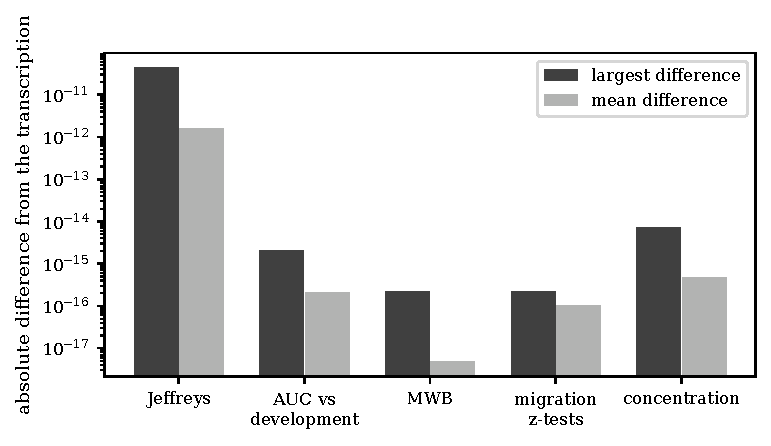
\includegraphics[width=0.8\textwidth]{ecb-agreement}
\caption{Largest and mean absolute difference between each ECB statistic of the engine and an independent transcription of the instructions, over \ecbInputs{} seeded random inputs per statistic, on a logarithmic axis; the Jeffreys bar is the accuracy of the quadrature used by the transcription.}
\label{fig:ecb-agreement}
\end{figure}

\subsection{The Jeffreys test against the nearest generic tests on the credit-card holdout}

On the \cCells{} grade cells of the eight models of the credit-card holdout (every grade with obligors, and the portfolio row of each model) the ECB Jeffreys test flags \flagJeffFive{} cells at the 5\,\% level and the exact one-sided binomial test of SciPy flags \flagBinFive{}; at the 1\,\% level both flag \flagJeffOne{}, so they differ in \disagreeFive{} cell at 5\,\% and in \disagreeOne{} at 1\,\%. The cell that differs is grade \diffGrade{} of the model \texttt{\diffModel{}}, with \diffN{} obligors and \diffD{} defaults, where the binomial $p$-value is \diffPb{} and the Jeffreys value \diffPj{}: the binomial value lies just above the level and the Jeffreys value just below, as Proposition~\ref{prop:sandwich} predicts, and no cell goes the other way. The Jeffreys interval of statsmodels, used as a one-sided limit at 5\,\%, reproduces the engine's decision on \smMatch{} of \cCells{} cells, so the building block exists in a statistics library and what the engine adds is the assembly: the grade-by-grade and portfolio tests with the obligor-weighted portfolio probability and the reporting fields. Figure~\ref{fig:jeffreys-binomial} plots the two $p$-values. The median absolute difference of the two is \medPGap{}, and the largest, \maxPGap{}, occurs in a grade of \worstGapN{} obligors with \worstGapD{} defaults of the model \texttt{\worstGapModel{}} where the two $p$-values are \worstGapPj{} and \worstGapPb{}; the sandwich bounds the difference by the probability of the observed count, which in a grade that small is large. The engine's values equal the committed $p$-values of the case to \committedGap{}. Hypothesis~H2 holds, narrowly: the two tests differ in one cell of \cCells{} at 5\,\% and in none at 1\,\%.

\begin{figure}[htbp]
\centering
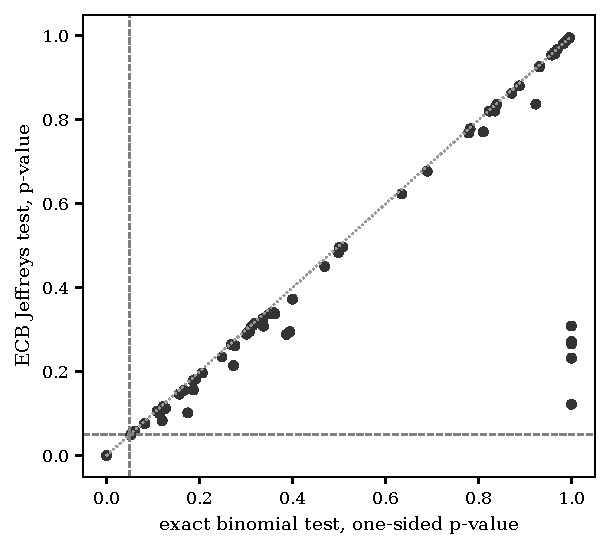
\includegraphics[width=0.55\textwidth]{jeffreys-binomial}
\caption{One-sided $p$-value of the ECB Jeffreys test against that of the exact binomial test for every grade cell of the eight credit-card models of the committed holdout; points lie on or below the diagonal as the sandwich of Proposition~\ref{prop:sandwich} requires, and dashed lines mark the 5\,\% level.}
\label{fig:jeffreys-binomial}
\end{figure}

\subsection{The portfolio engine against anchors, independent routes and its own rung}

The integral of the large-portfolio density equals the engine's distribution function to \lhpMax{} at seven points (Figure~\ref{fig:lhp-anchor}), which is the accuracy of the quadrature. The IRB capital of the credit-card book, at a default probability of \irbPd{} and correlation $0.04$, is \irbK{} by the formula written with SciPy, and the engine's IRB module and its large-portfolio capital differ from it by \irbDiff{}; the identity is exact because all three call the same normal distribution function, so the check holds the wiring and the formula and not the distribution function. The CreditRisk+ recursion returns a probability of no loss of \crpPzero{}, a mean of \crpMean{} loss units and a variance of \crpVar{}, and the variance differs from the closed form of Proposition~\ref{prop:crp} by a relative \crpVarGap{}, with \crpMass{} of probability mass beyond the grid of \crpNmax{} units at $\sigma^2=\crpSigma{}$. The independent recursion of \eqref{eq:crp}, written for the experiment, differs from the stable form by at most \crpIndMax{} in absolute terms over \crpCompared{} probabilities and by a relative \crpIndRel{} over the \crpIndPositive{} that are positive, which is the relative criterion of Hypothesis~H3, and from the engine's Panjer form by \crpIndPanjer{} in absolute terms. The granularity factor is $\delta=\gaDelta{}$ against the printed $4.83$, which agrees to the printed digits, and for identical names the product of the adjustment and the number of names is \gaTimesN{} at 10, 100, 1,000 and 10,000 names with a relative spread of \gaSpread{}.

\begin{figure}[htbp]
\centering
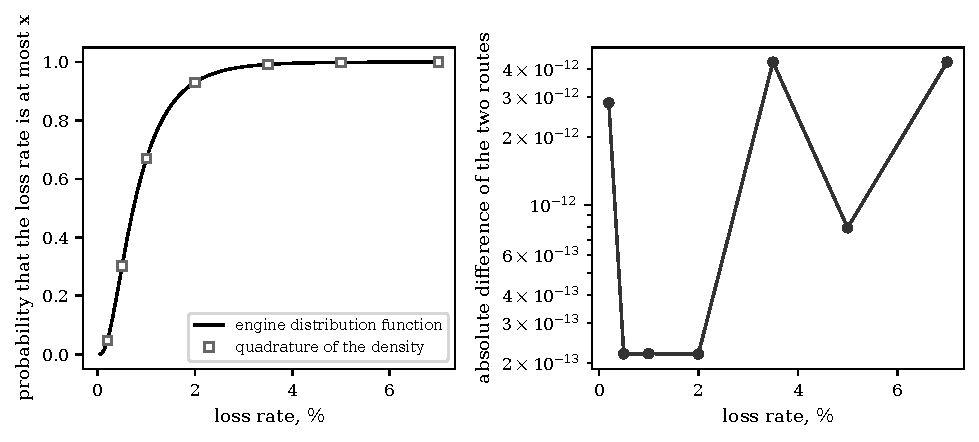
\includegraphics[width=\textwidth]{lhp-anchor}
\caption{Left: the distribution function of the large-portfolio loss rate at the fitted default probability and correlation of the commercial book, with the integral of the engine density computed by adaptive quadrature at seven points. Right: absolute difference of the two routes on a logarithmic axis.}
\label{fig:lhp-anchor}
\end{figure}

The copula sampler is compared with an independent simulator that draws its own normals. Over \mcReps{} runs of \mcScen{} scenarios each, at the correlation \mcRho{} of the one-factor rung, the 99\,\% value at risk is \mcVarNinetyNineEng{} $\pm$ \mcVarNinetyNineEngSd{} for the engine and \mcVarNinetyNineInd{} $\pm$ \mcVarNinetyNineIndSd{} for the independent simulator ($z=\mcVarNinetyNineZ{}$); the 99\,\% expected shortfall is \mcEsNinetyNineEng{} $\pm$ \mcEsNinetyNineEngSd{} and \mcEsNinetyNineInd{} $\pm$ \mcEsNinetyNineIndSd{} ($z=\mcEsNinetyNineZ{}$); the 99.9\,\% value at risk is \mcVarNinetyNineNineEng{} $\pm$ \mcVarNinetyNineNineEngSd{} and \mcVarNinetyNineNineInd{} $\pm$ \mcVarNinetyNineNineIndSd{} ($z=\mcVarNinetyNineNineZ{}$); and the 99.9\,\% expected shortfall is \mcEsNinetyNineNineEng{} $\pm$ \mcEsNinetyNineNineEngSd{} and \mcEsNinetyNineNineInd{} $\pm$ \mcEsNinetyNineNineIndSd{} ($z=\mcEsNinetyNineNineZ{}$). The mean loss is \mcMeanEng{} and \mcMeanInd{} against the exact expected loss of \mcElExact{}. All four $|z|$ values are below one, so the sampler agrees with the independent simulator within the resolution of Proposition~\ref{prop:power} (Figure~\ref{fig:mc-agreement}). The committed rung of \regenN{} scenarios at seed \regenSeed{} and chunk size \regenChunk{} is regenerated by the engine in \regenSeconds{} seconds with a largest relative difference of \regenRel{} over the eight values, the rounding of the committed file; the file holds rounded values, so the comparison cannot show equality of the unrounded sample. The Gaussian importance sampler estimates the probability that the loss exceeds the committed 99.9\,\% value at risk of \isThreshold{} as \isMean{} $\pm$ \isSd{} over \isReps{} seeds, against \isPlainMean{} $\pm$ \isPlainSd{} for plain sampling ($z=\isZ{}$, importance sampler minus plain sampling, the order of the other rows), with a variance ratio of \isRatio{} (Figure~\ref{fig:importance-sampling}); the expected-shortfall contributions of the groups sum to the sample expected shortfall of \eulerEs{} with a relative gap of \eulerGap{}. The Student $t$ importance sampler is not implemented, and the committed rung records that it did not run. Hypotheses~H3 and~H4 hold.

\begin{figure}[htbp]
\centering
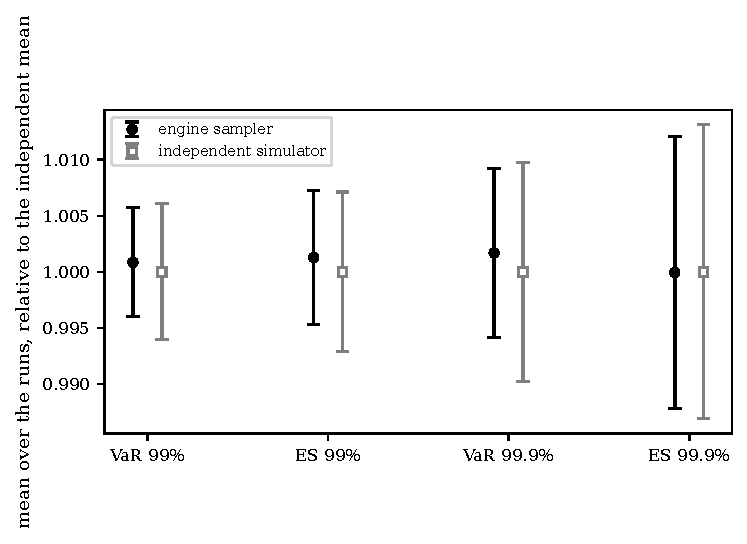
\includegraphics[width=0.8\textwidth]{mc-agreement}
\caption{Mean over \mcReps{} runs of the engine's copula sampler for four risk measures, relative to the mean of an independent simulator written from the model, with one standard deviation over the runs as the bar; the independent simulator sits at one by construction.}
\label{fig:mc-agreement}
\end{figure}

\begin{figure}[htbp]
\centering
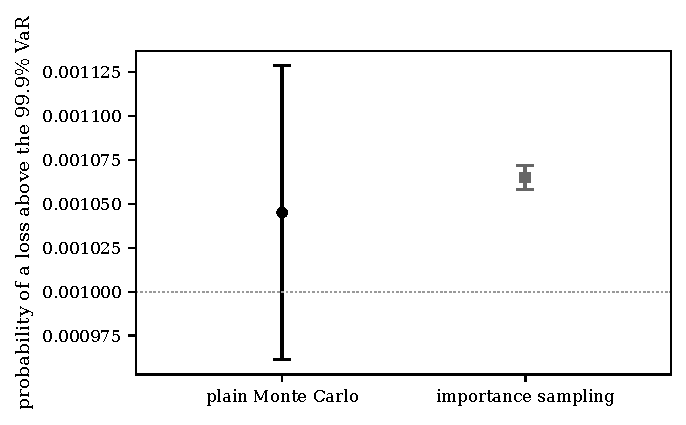
\includegraphics[width=0.6\textwidth]{importance-sampling}
\caption{Estimate of the probability that the portfolio loss exceeds the committed 99.9\,\% value at risk, from plain Monte Carlo and from the Gaussian importance sampler, as the mean over \isReps{} seeds of \isScen{} scenarios with one standard deviation as the bar; the dotted line is the nominal 0.1\,\%.}
\label{fig:importance-sampling}
\end{figure}

\subsection{The correlation estimator against a known truth}

Table~\ref{tab:grid} and Figure~\ref{fig:coverage-grid} give the coverage of the nominal 95\,\% interval in the committed simulator. The maximum-likelihood estimator has a mean coverage of \gridMlMeanCov{} over the \gridMlCells{} cells and its coverage is outside the 99\,\% band of $\pm\gridBandHalf{}$ in \gridMlFail{} of them: the lowest is \gridMlWorstCov{} at a true correlation of \gridMlWorstRho{} with series of \gridMlWorstYears{} years ($z=\gridMlWorstZ{}$). The coverage is below $0.95$ in \gridMlBelow{} of the \gridMlCells{} cells and the bias is negative in \gridMlNegBias{} of them, from \gridMlBiasMin{} to \gridMlBiasMax{}, so the estimator undercovers throughout the grid and not in one cell. Pooled over the \gridMlPooledReps{} replications of all cells the coverage lies $\gridMlPooledZ{}$ binomial standard errors from $0.95$, a figure that holds only if the cells are independent, which was not checked: one seed drives the 22-year grid. At a correlation of 0.24 and 22 years the coverage is \gridMlCovTwentyFour{} and the bias \gridMlBiasTwentyFour{}. The moments estimator has a mean coverage of \gridMomMeanCov{}, is outside the band in \gridMomFail{} of \gridMomCells{} cells, and its lowest coverage is \gridMomWorstCov{} at a correlation of \gridMomWorstRho{} with series of \gridMomWorstYears{} years; at 0.24 and 22 years its bias is \gridMomBiasTwentyFour{} and its coverage \gridMomCovTwentyFour{}. The re-run of three 22-year cells with \cellReps{} fresh replications gives coverages of \cellLowCov{} $\pm$ \cellLowCovSe{}, \cellMidCov{} $\pm$ \cellMidCovSe{} and \cellHighCov{} $\pm$ \cellHighCovSe{} at correlations of 0.02, 0.12 and 0.24, and biases of \cellLowBias{} $\pm$ \cellLowBiasSe{}, \cellMidBias{} $\pm$ \cellMidBiasSe{} and \cellHighBias{} $\pm$ \cellHighBiasSe{}. Hypothesis~H5 is refuted: \gridMlFail{} of \gridMlCells{} cells lie outside the band where \gridChance{} are expected by chance, and the mean coverage and the sign of the bias show an undercoverage that the single cell understates. The cell outside the band is the one at the lowest correlation with 22 years, and the re-run at that correlation is below $0.95$ as well.

\begin{table}[htbp]
\centering
\small
\caption{Coverage of the nominal 95\% interval at three of the twelve known correlations of the committed simulator, for 22 and 40 years, with 400 replications per cell; z is the distance of the coverage from 0.95 in binomial standard errors.}
\label{tab:grid}
\begin{tabular}{rrrrrr}
\toprule
Years & True correlation & ML coverage & z & Moments coverage & z \\
\midrule
22 & 0.020 & 0.912 & -3.441 & 0.823 & -11.700 \\
22 & 0.120 & 0.948 & -0.229 & 0.815 & -12.388 \\
22 & 0.240 & 0.940 & -0.918 & 0.655 & -27.071 \\
40 & 0.020 & 0.943 & -0.688 & 0.858 & -8.488 \\
40 & 0.120 & 0.940 & -0.918 & 0.870 & -7.341 \\
40 & 0.240 & 0.950 & 0.000 & 0.820 & -11.930 \\
\bottomrule
\end{tabular}
\end{table}


\begin{figure}[htbp]
\centering
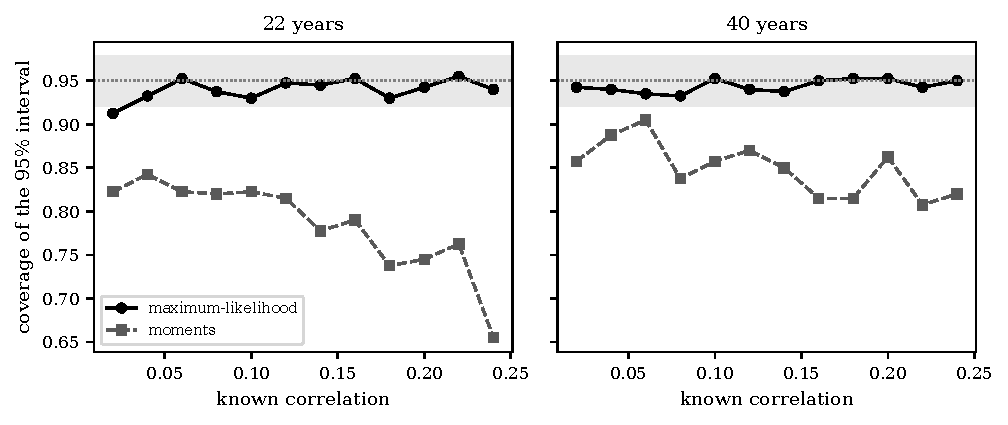
\includegraphics[width=\textwidth]{coverage-grid}
\caption{Coverage of the nominal 95\,\% interval of the asset correlation by the maximum-likelihood and the moments estimators against the known correlation of the committed simulator, for series of 22 and 40 years with \gridReps{} replications per cell; the shaded band is the 99\,\% binomial band around 0.95.}
\label{fig:coverage-grid}
\end{figure}

\subsection{The IRRBB engine against the standard and against QuantLib}

At a mid-point of 3.5 years the engine returns $\alpha_{\mathrm{s}}=\irrAlpha{}$, a short-up shock of \irrShort{} basis points, a steepener of \irrSteep{} and a flattener of \irrFlat{}, against the printed 0.417, 41.7, 25.4 and $-1.6$: the deviations are \irrAlphaDev{}, \irrShortDev{}, \irrSteepDev{} and \irrFlatDev{}, each inside the half-unit of the last printed digit (0.0005 for the factor and 0.05 basis points for the shocks). The transcription of the shocks written for the experiment equals the engine's values to the last digit shown. Over the \irrVariants{} committed variants, two currency legs and six shocks, that is \irrLegs{} leg and shock pairs, the shock shape stored in the artifact equals the engine's to \irrShapeEng{} and equals the transcription to \irrShapeInd{}; the engine's present value equals the stored one with a relative difference of \irrEngMax{}, as the artifact was written by the same function, and the QuantLib present value differs from the stored one by a relative \irrQlMax{} at most (Figure~\ref{fig:eve-reconciliation}). The pair rule that combines the peso and UF legs returns the stored value with a difference of \irrPair{}. Hypothesis~H6 holds, with the limit that QuantLib's present value is the same exponential discounting and so holds the time convention and the wiring of the engine and not the choice of continuous compounding.

\begin{figure}[htbp]
\centering
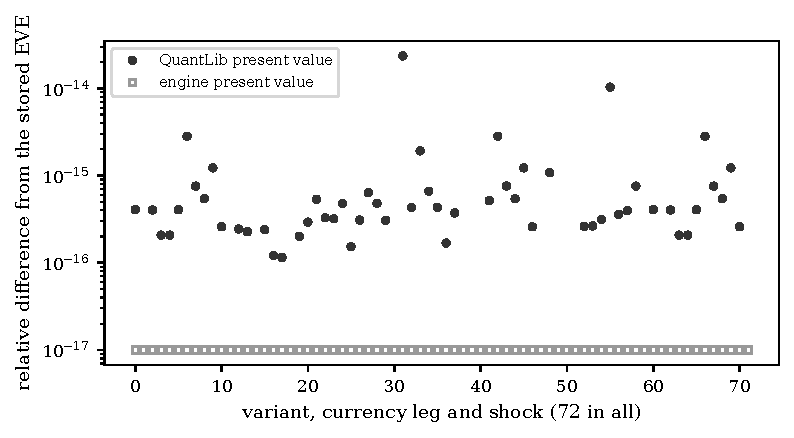
\includegraphics[width=0.85\textwidth]{eve-reconciliation}
\caption{Relative difference between the stored economic value of equity of each of the 72 leg and shock pairs of the six committed interest rate risk variants and the engine's present value and the QuantLib present value of the same cash flows, on a logarithmic axis; zero differences are drawn at the axis floor.}
\label{fig:eve-reconciliation}
\end{figure}

\subsection{The open toolkits}

The survey queried \pypiQueried{} package names on \pypiDate{}, of which \pypiFound{} exist on PyPI; the \pypiMissing{} that do not are \pypiMissingNames{}. Table~\ref{tab:toolkits} sets the vocabulary of the catalogue against the \distScanned{} installed distributions, whose \filesScanned{} Python files were scanned, and against the summary and long description of the \pypiFound{} packages. In the installed sources the word Jeffreys appears in the statistics library for the proportion and rate intervals, Herfindahl in the binning library for a concentration index of the bins, Vasicek in the SciPy entropy estimator of that name and not in the credit model, and the weighted-matrix words in a graph test. In the package texts, the only package that names the Jeffreys test, CreditRisk+, the granularity adjustment, the Vasicek model, the ECB or the interest rate risk in the banking book is the engine itself. Hypothesis~H7 is not refuted by this survey; its limits are those of a search of metadata and of an installed environment, and Section~\ref{sec:limitations} states them.

\begin{table}[htbp]
\centering
\small
\caption{Where the catalogue's vocabulary appears in the Python sources of 106 installed distributions and in the PyPI summary and description of 34 toolkits read on 2026-11-06; a match is a word, not an implementation of the specified test.}
\label{tab:toolkits}
\begin{tabular}{lrlrl}
\toprule
Vocabulary & Installed packages with a match & Which & PyPI texts with a match & Which \\
\midrule
jeffreys & 1 & statsmodels & 1 & riskvalidation \\
herfindahl & 1 & optbinning & 0 & -- \\
matrix weighted bandwidth & 1 & networkx & 0 & -- \\
creditrisk+ & 0 & -- & 1 & riskvalidation \\
granularity adjustment & 0 & -- & 1 & riskvalidation \\
vasicek & 1 & scipy & 1 & riskvalidation \\
irrbb & 0 & -- & 1 & riskvalidation \\
economic value of equity & 0 & -- & 0 & -- \\
somers d & 2 & scipy, statsmodels & 0 & -- \\
migration matrix test & 0 & -- & 0 & -- \\
\bottomrule
\end{tabular}
\end{table}


\section{Ablation}
\label{sec:ablation}

Table~\ref{tab:ablation} lists the \ablMutants{} defects planted in the released engine and the layers that detect each, and Figure~\ref{fig:ablation-matrix} draws the same matrix. The engine as released passes all five layers (\ablFalseAlarms{} false alarms), and passes them again after the last defect is removed; a false alarm at either point would have stopped the run. A layer detects a defect only when one of its checks fails. An exception raised while a layer runs, such as an exhausted memory, is a failed run: the script runs the layer again and, if the exception persists, stops without writing a result, and in the committed run a layer was run again after an exception \ablRetriesCommitted{} times, and the committed matrix was reproduced cell for cell by \ablReproduced{} of \ablReruns{} further runs of the script (Section~\ref{sec:reproducibility}). The rule matters because an earlier version of the script recorded an exception as a detection; on a loaded machine a rerun of that version, by a reader other than the writer, recorded four detections that were memory errors, in layers $C$ and $E$, and with them layer $D$ had no unique detection and Hypothesis~H8 failed. Ten of the defects change a result of the engine; two (a different seed and a different chunk size of the sampler) change the sample path and not its distribution, and are labelled equivalent in the table.

\begin{table}[htbp]
\centering
\small
\caption{Defects planted one at a time in the released engine and the verification layers that detect each: A analytic anchors, B published vectors and the ECB transcription, C regeneration of the committed rung, D known-truth simulator, E cross-implementation; x marks a detection.}
\label{tab:ablation}
\begin{tabular}{lp{6.4cm}cccccc}
\toprule
Id & Defect planted in the engine & Equivalent & A & B & C & D & E \\
\midrule
P01 & granularity delta scaled by 1.02 & no & . & x & . & . & . \\
P02 & large-portfolio distribution function with the correlation scaled by 1.05 & no & x & . & . & . & . \\
P03 & copula sampler drawn with the next seed (statistically equivalent) & yes & . & . & x & . & . \\
P04 & copula loadings scaled by 0.97 (correlation 6 percent low) & no & . & . & x & . & . \\
P05 & CreditRisk+ recursion shifted by one loss unit & no & x & . & . & . & x \\
P06 & Jeffreys prior Beta(1, 1) in place of Beta(1/2, 1/2) & no & . & x & . & . & . \\
P07 & concentration statistic with sqrt(K) in place of sqrt(K-1) & no & . & x & . & . & . \\
P08 & flattener long coefficient 0.65 in place of 0.60 & no & . & x & . & . & x \\
P09 & present value with annual compounding in place of continuous & no & . & . & . & . & x \\
P10 & maximum-likelihood correlation scaled by 0.7 & no & . & . & . & x & . \\
P11 & large-portfolio capital scaled by 1.01 & no & x & . & . & . & . \\
P12 & copula sampler ignores the committed chunk size (statistically equivalent) & yes & . & . & x & . & . \\
 & Detections of the defects that change a result &  & 3 & 4 & 1 & 1 & 3 \\
\bottomrule
\end{tabular}
\end{table}


\begin{figure}[htbp]
\centering
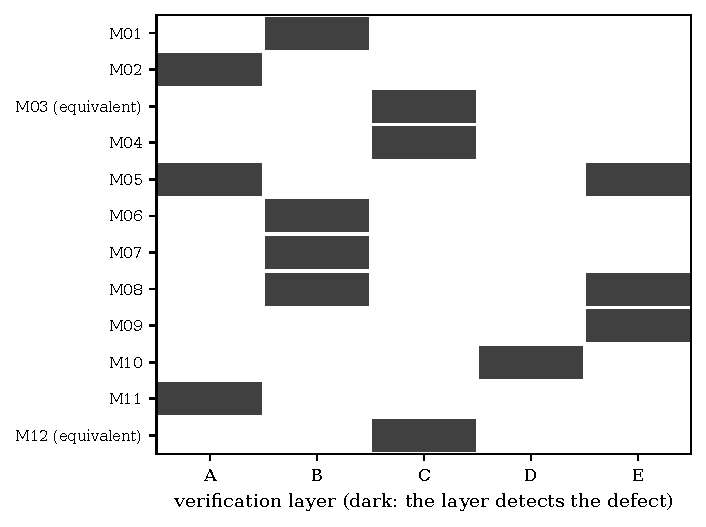
\includegraphics[width=0.62\textwidth]{ablation-matrix}
\caption{Detection matrix of the \ablMutants{} planted defects (rows) by the five verification layers (columns): a dark cell means the layer detects the defect; the two defects labelled equivalent change the sample path of the sampler and not its distribution.}
\label{fig:ablation-matrix}
\end{figure}

\subsection{What each layer contributes}

Layer A, the analytic anchors, detects \ablAReal{} of the \ablReal{} defects that change a result. It finds the correlation scaled in the large-portfolio distribution function (found by: \ablDetTwo{}), the recursion shifted by one loss unit (\ablDetFive{}) and the large-portfolio capital scaled by one per cent (\ablDetEleven{}). Layer B, the published vectors and the ECB transcription, detects \ablBReal{}: the granularity factor scaled by 1.02 (\ablDetOne{}), the Jeffreys prior changed from one half to one (\ablDetSix{}), the concentration statistic with the wrong square root (\ablDetSeven{}) and the flattener coefficient (\ablDetEight{}); none of these four moves a quantity that the anchors evaluate. Layer C, the regeneration of the committed rung, detects \ablCAll{} defects of the twelve, which are the two defects that change the sample path without changing the distribution and the loading defect (\ablDetFour{}); of the real defects it detects \ablCReal{}. Layer D, the known-truth simulator, detects \ablDReal{}: the maximum-likelihood correlation scaled by 0.7 (\ablDetTen{}), which no arithmetic check evaluates. Layer E, the cross-implementation checks, detects \ablEReal{}: the recursion shift (\ablDetFive{}), the flattener coefficient (\ablDetEight{}) and the annual compounding that replaces the continuous one (\ablDetNine{}); the last is found by no other layer.

\subsection{The unique detections and the equivalent defects}

\ablAny{} of the \ablReal{} real defects are detected by at least one layer, \ablOnly{} by exactly one, and \ablNone{} by none. Each layer detects a real defect that no other layer detects: the distribution function and the capital scaled by a constant for the anchors, the granularity, the prior and the concentration square root for the vectors, the loading defect for the regeneration, the biased estimator for the known-truth simulator and the compounding rule for the cross-implementation layer. Hypothesis~H8 therefore \ablHEight{}: \ablLayersWithUnique{} of the five layers have a unique detection (layer $A$ \ablAUnique{}, $B$ \ablBUnique{}, $C$ \ablCUnique{}, $D$ \ablDUnique{} and $E$ \ablEUnique{}). The hypothesis measures how far the check sets cover the engine: each unique detection follows from the engine function that the layer exercises and that no other layer calls (Section~\ref{sec:limitations}), and only two defects are seen by two layers. The two equivalent defects are detected by layer C and by no other, \ablCEquiv{} of \ablEquiv{}: the regeneration check is a regression check, since it signals any change in the sequence of random numbers that the committed result was generated from, whether or not the change matters to the engine's statistics, and a signal from it that no other layer confirms calls for a decision about whether the change is a defect and not for a fix.

\subsection{The loading defect against the resolution of the cross-implementation layer}

The one real defect that only the regeneration found is the scaling of the copula loadings by \effLoadingFactor{}, which lowers the asset correlation by \effCorrPct{} per cent. At the size of the main comparison it moves the 99\,\% value at risk of the engine by \effChangeVarNinetyNine{}\,\%, the 99\,\% expected shortfall by \effChangeEsNinetyNine{}\,\%, the 99.9\,\% value at risk by \effChangeVarNinetyNineNine{}\,\% and the 99.9\,\% expected shortfall by \effChangeEsNinetyNineNine{}\,\% (mean over \effReps{} seeds of \effScen{} scenarios, against the engine without the defect). The cross-implementation layer compares three runs of 40,000 scenarios for each route on the 99\,\% value at risk and rejects at four standard errors, so by Proposition~\ref{prop:power}, with $c=4$ and the run-to-run error scaled with the square root of the number of scenarios and runs, its minimum detectable shift at a power of $0.8$ is \effMddVarNinetyNine{}\,\% of the 99\,\% value at risk; a Student distribution with four degrees of freedom would make it larger still. The shift of the defect, \effChangeVarNinetyNine{}\,\%, is below that resolution, so the layer as run cannot detect it, and it does not.

At the size of the main comparison the minimum detectable shifts at the cutoff $c=3$ of Hypothesis~H3 are \mcMddVarNinetyNine{}, \mcMddEsNinetyNine{}, \mcMddVarNinetyNineNine{} and \mcMddEsNinetyNineNine{}\,\% of the four measures. The defect was run at that size: \fsReps{} runs of \fsScen{} scenarios of the defective engine, compared with the stored runs of the independent simulator of Section~\ref{sec:results}. The shifts from the independent simulator are \fsShiftVarNinetyNine{}, \fsShiftEsNinetyNine{}, \fsShiftVarNinetyNineNine{} and \fsShiftEsNinetyNineNine{}\,\%, and $z=\fsZVarNinetyNine{}$, $\fsZEsNinetyNine{}$, $\fsZVarNinetyNineNine{}$ and $\fsZEsNinetyNineNine{}$ for the 99\,\% value at risk, the 99\,\% expected shortfall, the 99.9\,\% value at risk and the 99.9\,\% expected shortfall (defective engine minus independent simulator). The full-size comparison therefore rejects the engine on \fsFlagged{} of the four measures by the criterion $|z|\le3$ of Hypothesis~H3 and misses it on the 99.9\,\% expected shortfall, whose minimum detectable shift is close to the shift the defect produces there. The conclusion is not that the independent simulator is weak, but that its resolution is a number that Proposition~\ref{prop:power} computes, that a validator can choose by the number of runs and of scenarios, and that one defect at one size illustrates it and does not map it.

\section{Discussion}
\label{sec:discussion}

\subsection{What the agreement does and does not establish}

Every implemented component agrees with its independent reference to the accuracy of the reference: the five ECB statistics to \ecbAllMax{}, the large-portfolio law to \lhpMax{}, the CreditRisk+ recursion to \crpIndMax{} against an independent recursion, the copula sampler to within a $|z|$ below one against an independent simulator, and the interest rate present values to \irrQlMax{} against QuantLib. These are necessary conditions. A defect that the engine and its reference share, a wrong reading of a specification, or an error in a region of the input space that no reference visits, would pass every check of Section~\ref{sec:results}. The checks are strongest where the reference differs most from the component: the transcription of the ECB statistics uses loops and a quadrature where the engine uses vectorised code and a library distribution function, and an independent simulator draws its own random numbers. They are weakest where the reference is the same arithmetic, as in the IRB formula and the QuantLib present value, and the manuscript says so where it reports them. The measured scope of the catalogue is narrower than a reading of its title suggests. The engine implements \ecbImpl{} of the \ecbSections{} statistics that the ECB instructions fix, all of them on the probability of default, and none on the loss given default, the credit conversion factor or the exposure at default beyond a related two-sided paired $t$-test; a validator who needs the ECB's loss-side statistics as specified does not find them in this engine.

\subsection{The Jeffreys test as an assembly, not a new statistic}

The Jeffreys test is a Beta distribution function evaluated at the applied probability, and Proposition~\ref{prop:sandwich} places it between two binomial tails. On the grades of the credit-card holdout this means the generic tests give nearly the same decisions: \flagJeffFive{} cells flagged against \flagBinFive{} at 5\,\% and none different at 1\,\%, and the statsmodels interval reproduces the engine's decision in every cell. The reason to use the engine's test is therefore not the arithmetic. It is that the grade-by-grade tests and the portfolio test are produced together, with the obligor-weighted portfolio probability that the instructions require, in the result record that carries the null hypothesis, the primary source and the policy, so that a report assembled from them is the report the instructions describe. A reader who expects a different statistic from the Jeffreys test than from the binomial test in a large grade will not find one, and Proposition~\ref{prop:sandwich} says why: the difference is bounded by the probability of the observed count. The substitution is not free in a small grade, where the largest difference between the two $p$-values is \maxPGap{}; but it is conservative, because the binomial test cannot flag a grade that the ECB test passes.

\subsection{Why the five layers are different layers}

The ablation of Section~\ref{sec:ablation} shows that each layer sees a different part of the engine. The analytic anchors see the distribution functions and the recursion and are blind to the sampler and to the tests. The published vectors and the ECB transcription see constants, priors and coefficients that a formula carries, and nothing that depends on a seed. The regeneration of the committed rung sees every change of the sampler's sample path, including those that are not defects, and for that reason it is a regression check and not a correctness check; it was the only layer to find the loading defect, whose size is given in Section~\ref{sec:ablation}. The known-truth simulator sees a biased estimator that no arithmetic check can see, since the defect is in the estimator's output and not in a formula the other layers evaluate. The cross-implementation layer sees the compounding rule that a formula-level check does not exercise, and it has a resolution that Proposition~\ref{prop:power} quantifies. No layer is redundant in the \ablReal{} defects tried, and no layer is sufficient: \ablNone{} real defect is found by none, and the others are found by between one and two layers.

\subsection{Negative results and failure cases}

Four results go against a simple reading. The correlation interval does not cover as claimed in the cell at the lowest correlation and the shortest series, with a coverage of \gridMlWorstCov{} against a nominal $0.95$; the moments estimator is outside the band in \gridMomFail{} of \gridMomCells{} cells, so its interval should not be read as a 95\,\% interval anywhere in the grid. The engine's absent ECB statistics are a negative result about the catalogue, not about any test. The Student $t$ importance sampler does not exist and the rung says so. And the one comparison in which a defect of $6\,\%$ in the correlation passes a cross-implementation check at the size run in the ablation is a statement about that layer's resolution and about the choice of its size, not about the engine. A validator who uses the layers should read them as the table of Section~\ref{sec:ablation} suggests: the five together find what each alone misses, and the absence of a finding is a statement about the references used.

\section{Limitations}
\label{sec:limitations}

\subsection{Internal validity}

Agreement between two routes shows that they compute the same thing, not that the thing is the right one. Three of the checks hold less than they appear to. The IRB capital of the credit-card book is equal to the SciPy formula to the last digit because the engine and the formula call the same normal distribution function, so the check holds the wiring of the formula and nothing about the distribution function. The QuantLib present value is the same exponential discounting as the engine's and agrees to \irrQlMax{}; it holds the time convention and the bucket wiring and not the choice of continuous compounding, and the defect of the ablation that replaces it by annual compounding is found for that reason and not because QuantLib is an independent model of the cash flows. The Jeffreys transcription is accurate to \ecbJeffMax{}, the accuracy of a quadrature, so a defect smaller than that in the engine's Beta function call would pass. A second limit is that the transcription of the ECB statistics was written for this study from the specification as extracted, and a misreading of the specification that was shared by the engine and the transcription would pass both; the specification's loss and exposure formulas were not transcribed because the engine does not implement them. The ablation's defects were chosen by the experimenter and are \ablMutants{} in number, so the detection counts describe those defects and are not an estimate of the detection rate over the defects that a developer makes. Layer B applies the transcription to the Jeffreys and the concentration statistics only, and layer E runs at reduced size, so their detections understate what the full experiments of Section~\ref{sec:results} would find.

\subsection{External validity and scope}

The real-outcome data are the credit-card holdout, used for the Jeffreys comparison, and the charge-off rates that fit the loan book; the loan book itself is constructed and the interest rate risk bank is synthetic, so no result concerns the model of an actual bank. The portfolio checks cover one book of \(1{,}120\) names and one correlation structure in one sector for the CreditRisk+ recursion; multi-sector recursions, random loss given default, the Student $t$ copula's importance sampler and migration-mode models are not implemented or not checked. The correlation grids are read as committed and only three cells were re-run, with \cellReps{} replications each, so the cell that falls outside the band is known to fall outside from the committed 400 replications and is confirmed in direction, not in size, by the re-run. The shock-size tables of the IRRBB engine are not compared in this study with the primary tables of the standard; only the worked example is. The ECB statistics for the loss given default and the exposure parameters are absent from the engine, and the statement of Section~\ref{sec:results} that the package implements the probability-of-default statistics is a statement about the registry at one release. The list of the \ecbSections{} statistics is the author's reading of Sections 2.4 to 2.10 of the instructions; for the slotting section only the headings were read and not the content, so whether it fixes a statistic that could be implemented is not confirmed, and the count of absent statistics depends on counting that section and the qualitative process statistics as one entry each.

\subsection{Construct validity and the absence claim}

The motivating claim that no open toolkit implements these tests as specified is a claim of absence, and absence is established only for the places searched. The survey read the metadata (summary and long description) of \pypiFound{} packages from a list written by the authors, on \pypiDate{}; a package that implements a test without naming it in its description would not be found, a package outside the list would not be found, and GitHub was not searched by this study. The scan covers the Python sources of the installed distributions of one environment; compiled modules, such as the QuantLib core, are not scanned. The earlier search that the claim rests on, of GitHub and PyPI on the 4th of October 2026 and of CRAN and GitHub for portfolio models, is not repeated here, and the claim is stated as holding for maintained, permissively licensed implementations on those dates. The $z$ comparisons use the normal approximation with \mcReps{} runs, for which a Student distribution would give wider limits; the largest $|z|$ reported is below one, so the conclusion does not depend on it, but the minimum detectable shifts of Proposition~\ref{prop:power} are approximate. Finally, the 99\,\% band used for the coverage cells treats the 24 cells as independent comparisons with no correction for multiplicity; with a Bonferroni correction over 24 cells at a family-wise level of 5\,\% the cutoff of $|z|$ is 3.08 and the cell at $z=\gridMlWorstZ{}$ still lies outside it, but at a family-wise level of 1\,\% the cutoff is 3.53 and it lies inside. The refutation of Hypothesis~H5 therefore holds at the level at which the hypothesis was stated and is not robust to a stricter family-wise correction.

\section{Reproducibility}
\label{sec:reproducibility}

The source code, the committed data and the computational outputs are in the repository \texttt{github.com/fsantibanezleal/CAOS\_Contraste}, under \texttt{manuscripts/engines-and-test-catalogues}, release v1.00.000 of CAOS\_Contraste (tag \texttt{v1.00.000}); the engine is the package \texttt{riskvalidation} release \inventoryVersion{} on PyPI, installed with its market, machine-learning and stress extras, together with NumPy, SciPy, statsmodels, QuantLib and Matplotlib~\citep{harris2020,virtanen2020,seabold2010,hunter2007}. The committed artifacts read by the experiments are the documents under \texttt{data/derived} of the credit-card, portfolio-capital and interest-rate-risk cases, each with its provenance and the engine release that wrote it. % voice-ok: citation of the product release the results were produced with

Six scripts under \texttt{experiments} produce the results, each writing a JSON file next to it with the wall time and peak memory of its run, and two scripts under the manuscript folder write the tables and figures:
\begin{itemize}
\item \texttt{run\_ecb.py} writes \texttt{results\_ecb.json}: the differential tests of the five ECB statistics (seed 20261105) and the Jeffreys comparison on the credit-card holdout;
\item \texttt{run\_portfolio.py} writes \texttt{results\_portfolio.json}: the anchors, the independent simulator (seeds 910001 onward), the regeneration of the committed rung, the grids, the re-run cell (seed 20261106) and the importance sampler (seeds 777000 and 888000 onward);
\item \texttt{run\_irrbb.py} writes \texttt{results\_irrbb.json}: the worked example, the shock transcription and the QuantLib present values;
\item \texttt{run\_catalogue.py} writes \texttt{results\_catalogue.json}: the registry, the ECB coverage, the scan of the installed sources and the survey of the package index, which is cached and kept with \texttt{--offline};
\item \texttt{run\_ablation.py} writes \texttt{results\_ablation.json}: the planted defects and the five layers (seed 20261107); an exception raised by a layer is retried and, if it persists, stops the run without writing a result;
\item \texttt{run\_ablation\_effect.py} writes \texttt{results\_ablation\_effect.json}: the size of the copula-loading defect on the four risk measures over five seeds (seeds 31000 onward) and its comparison with the independent simulator at the size of the main comparison, ten runs of 200,000 scenarios (seeds 32000 onward);
\item \texttt{make\_tables.py} and \texttt{make\_figures.py} write every table, every figure and the file \texttt{tables/numbers.tex}, which defines one macro for each number quoted in the prose, so that the text carries no number typed by hand; \texttt{number\_sources.py} lists each macro with the sections that use it and its source.
\end{itemize}
\begin{table}[htbp]
\centering
\small
\caption{Wall time and peak resident memory of one run of each experiment script, as recorded in the \texttt{run} field of its results file, on the machine described in Section~\ref{sec:reproducibility}.}
\label{tab:runs}
\begin{tabular}{llrr}
\toprule
Script & Writes & Wall time & Peak memory (MB) \\
\midrule
\texttt{run\_ecb.py} & \texttt{results\_ecb.json} & 30 s & 139 \\
\texttt{run\_irrbb.py} & \texttt{results\_irrbb.json} & under 1 s & 127 \\
\texttt{run\_catalogue.py} & \texttt{results\_catalogue.json} & 10 min & 139 \\
\texttt{run\_portfolio.py} & \texttt{results\_portfolio.json} & 35 min & 1,129 \\
\texttt{run\_ablation.py} & \texttt{results\_ablation.json} & 21 min & 423 \\
\texttt{run\_ablation\_effect.py} & \texttt{results\_ablation\_effect.json} & 3 min & 211 \\
\bottomrule
\end{tabular}
\end{table}


Each script is run from the repository root with the interpreter of the environment (\texttt{python manuscripts/engines-and-test-catalogues/experiments/run\_ecb.py}, and likewise for the others), and the document is built with two passes of \texttt{pdflatex} around \texttt{bibtex}. The scripts were run on a laptop with an Intel Core i9-14900HX processor (24 cores, 32 threads) and 48 GB of memory under Windows 11 with Python \runPython{}. Table~\ref{tab:runs} gives the wall time and the peak resident memory of one run of each script, taken while two of the scripts ran at the same time on the machine, so that the times are upper bounds; the largest peak is \runPeakMax{} MB, and the regeneration of the committed rung alone takes \regenSeconds{} seconds. The ablation repeats the regeneration for every defective engine and is the longest script after the portfolio script. The tests of the measurement code, \texttt{test\_run\_ablation.py}, \texttt{test\_run\_ablation\_effect.py} and \texttt{test\_run\_catalogue.py}, are run with \texttt{pytest} from the repository root on the \texttt{experiments} folder of the manuscript. \ablRerunSentence{} The seeds are listed above, the number of repetitions in Section~\ref{sec:experimental-design}, and the survey carries its date, so a rerun of the survey on another day may find other package versions and is not expected to reproduce its counts.

The identifiers of the computations in this paper are the names of the committed scripts and of the keys of their JSON outputs; the macros of \texttt{numbers.tex} are each preceded by a comment that names the key from which the number comes. No external data are downloaded by the analyses except the package metadata of the survey.

\section{Conclusions}
\label{sec:conclusions}

The open package studied here holds \testsTotal{} registered tests, five of the \ecbSections{} statistics of the European Central Bank's instructions for reporting the validation of internal credit models, a copula and CreditRisk+ portfolio engine and an engine for interest rate risk in the banking book, and each implemented component agrees with a reference that shares none of its code.
The five ECB statistics agree with an independent transcription of the instructions to \ecbAllMax{} on \ecbInputs{} random inputs each, the large-portfolio law to \lhpMax{}, the CreditRisk+ recursion to \crpIndMax{} against an independent recursion, the copula sampler within $|z|<1$ of an independent simulator over \mcReps{} runs of \mcScen{} scenarios, the committed one-million-scenario rung to a relative \regenRel{}, and the interest rate present values to a relative \irrQlMax{} against QuantLib on \irrLegs{} leg and shock pairs (Table~\ref{tab:main-results}).
Hypotheses~H1 (first part), H2, H3, H4, H6, H7 and H8 held; the second part of Hypothesis~H1 and Hypothesis~H5 did not.

Three results limit what the package can be said to offer.
First, \ecbAbsent{} of the \ecbSections{} ECB statistics are not implemented (the qualitative process statistics, the loss, conversion factor and exposure statistics, and the slotting statistics), so a validator who needs the loss-side statistics as specified does not find them here.
Second, the Jeffreys test differs from the exact binomial test in \disagreeFive{} of \cCells{} grade cells of eight credit-card models at the 5\,\% level and in none at the 1\,\%, which Proposition~\ref{prop:sandwich} explains: the engine's contribution is the assembly of the grade and portfolio tests in one result record, not a new statistic.
Third, the maximum-likelihood interval of the asset correlation falls outside the binomial band of its simulator in \gridMlFail{} of \gridMlCells{} cells, at a correlation of \gridMlWorstRho{} with series of \gridMlWorstYears{} years, and the refutation does not survive a Bonferroni correction at a family-wise level of 1\,\%.

The protocol that produced these agreements was itself measured.
Of \ablMutants{} planted defects, \ablReal{} change a result; \ablAny{} of them are found by at least one of the five layers and \ablOnly{} by exactly one, and each layer finds a defect that no other layer finds.
The regeneration of a committed result flags the two changes of the sample path that are not defects, so it is a regression check and not a correctness check, and a cross-implementation check at reduced size cannot see a six per cent defect in the correlation that the full-size comparison would see, because the resolution of an independent simulation is a number that Proposition~\ref{prop:power} computes.
The absence claim that motivated the package, that no open toolkit implements the specified tests, is not refuted by a survey of \pypiFound{} package descriptions and \distScanned{} installed distributions and is not proved by it.

Four pieces of work follow from these limits.
The ECB statistics of the loss given default, the credit conversion factor and the exposure have to be transcribed from the instructions and implemented, and the transcription written for this study is the template for checking them.
The CreditRisk+ checks have to be extended to several sectors and to an idiosyncratic weight, where the recursion has more terms and Proposition~\ref{prop:crp} does not apply.
The correlation estimator needs an interval that covers at short series and low correlations, and the moments estimator needs one that covers anywhere in the grid.
The absence claim needs a search that reads source code and not only package descriptions, repeated on a stated date, before it is stated without the limits of Section~\ref{sec:limitations}.
Until then, the supported statement is narrower than the title of a catalogue: the components listed in Table~\ref{tab:main-results} reproduce what exists outside the package to the stated accuracy, and the checks that show it are a necessary condition for the correctness of an engine, not a sufficient one.


\bibliographystyle{plainnat}
\bibliography{references}

\end{document}
